\documentclass[11pt]{article}

% =====================================================================
% WARNING: OBSOLETE DRAFT — SUPERSEDED BY main.tex
% =====================================================================
% This file is an early working draft retained for reference only.
% All numerical results, tables, and figures herein have been
% superseded by the final version in paper/main.tex.
% Do not cite, distribute, or use for evaluation.
% =====================================================================

% -----------------------------
% Packages (minimal, common)
% -----------------------------
\usepackage[a4paper,margin=1in]{geometry}
\usepackage{microtype}
\usepackage{hyperref}
\usepackage{enumitem}
\usepackage{graphicx}
\usepackage{booktabs}
\usepackage{amsmath,amssymb}
\usepackage{tikz}
\usetikzlibrary{shapes.geometric, shapes.symbols, arrows.meta, positioning, fit, backgrounds, calc}
\usepackage{float}

% -----------------------------
% Metadata
% -----------------------------
\title{STREAMTRACK: Multi-Camera Object Tracking Using Streams and Tables}
\author{Mahmoud Tayee, Ahmed Awad}
\date{\today}

\begin{document}
\maketitle

\begin{abstract}
Multi-camera object tracking (MCOT) is typically implemented as a tightly coupled computer-vision pipeline, making it difficult to scale cross-camera association, to inspect intermediate decisions, and to adapt to changes in the camera network. This paper presents an alternative systems-oriented formulation: MCOT as a streaming program in which detections and tracklet updates are streams, identity hypotheses are maintained as relational state tables, and cross-camera association is expressed as continuous SQL/EPL queries. Inter-camera tracking is realised via topology-aware stream joins parameterised by a dynamically updateable camera neighbourhood table. Our results demonstrate that this relational approach achieves a \textbf{156$\times$ average speedup} in the core similarity generation stage and a \textbf{34$\times$ overall speedup} relative to conventional batch-oriented baselines. Furthermore, scaling the system to 9 cameras with topology-aware partitioning yields an additional \textbf{4.16$\times$} latency reduction (up to \textbf{4.27$\times$} in steady state excluding JVM warm-up) per association call, while providing an architecture that supports zero-downtime reconfiguration of the camera neighborhood topology.
\end{abstract}

\section{Introduction}
\subsection{Motivation}
Multi-camera object tracking is essential for modern AI applications such as smart retail monitoring, urban traffic management, and airport security. However, these systems must simultaneously satisfy (i) computer-vision accuracy requirements and (ii) operational requirements such as scalability, debuggability, and reconfigurability. Conventional implementations often embed cross-camera association logic into bespoke code, which complicates maintenance and makes runtime changes (e.g., adding a camera or redefining neighborhood links) disruptive and resource-intensive.

\subsection{Key Insight}
We recast MCOT as a \emph{streams-and-tables} program: (a) \emph{streams} represent observations and incremental tracklet hypotheses; (b) \emph{tables} represent persistent state (tracklets, global identities, and the camera network topology); and (c) continuous SQL/EPL queries implement the operator graph that transforms per-camera observations into a unified, globally consistent identity track.

\subsection{Contributions}
\begin{itemize}[leftmargin=*]
    \item An operator-graph formulation of MCOT using streams and relational state tables.
    \item An end-to-end SQL/EPL realization over a CEP/streaming engine (Esper), including streaming counterparts of key clustering/association components.
    \item Topology-aware cross-camera association expressed as stream joins, reducing candidate comparisons relative to naive all-pairs matching.
    \item A dynamically updateable camera neighborhood topology table that provides an architecture for runtime reconfiguration without code changes or pipeline resets.
    \item A performance-optimized implementation (\textbf{Ours}) that achieves a \textbf{156$\times$ average speedup} in the primary similarity generation stage and a \textbf{34$\times$ overall speedup} relative to the batch baseline (\textbf{Theirs}). This is realized through a two-stage enhancement: (1) a migration to a \textbf{relational streams-and-tables architecture} that yields an architectural speedup in coordinate projection and state maintenance, and (2) \textbf{Topology-Aware Stream Join} optimization that delivers a \textbf{4.16$\times$} latency reduction (up to \textbf{4.27$\times$} in steady state excluding JVM warm-up) when scaling to 9 cameras.
\end{itemize}

\subsection{Paper Organization}
Section~\ref{sec:background} defines the problem and background. Section~\ref{sec:overview} presents the system overview and data model. Sections~\ref{sec:operators}--\ref{sec:joins} detail the operator graph and topology-aware joins. Section~\ref{sec:implementation} outlines the SQL/EPL implementation. Section~\ref{sec:evaluation} describes the evaluation plan. Sections~\ref{sec:discussion}--\ref{sec:conclusion} conclude with discussion, related work, and future directions.

\section{Background and Problem Definition}\label{sec:background}
\subsection{Multi-Camera Object Tracking (MCOT)}
We consider a set of cameras $\mathcal{C} = \{c_1,\dots,c_m\}$. Each camera produces a stream of detections $\mathcal{D}_c$, where each detection $d \in \mathcal{D}_c$ consists of a bounding box, an appearance embedding vector $f \in \mathbb{R}^d$, and a timestamp $t$. The goal of MCOT is to assign a \emph{global identity} $ID_G$ to each observation such that all detections of the same physical object across the camera network $\mathcal{C}$ share the same identity over time, producing consistent and continuous identity tracks.

\subsection{Baseline Pipeline (Starting Point)}
We begin from a representative multi-camera tracking pipeline that (i) constructs tracklets per camera (Single-Camera Tracking), (ii) selects representative visual features for each track (Representative Selection), (iii) performs cross-camera re-identification (Re-ID) via similarity-based clustering, and (iv) assigns lower-confidence detections in a post-processing stage. Our work re-architects this functional intent as a streaming operator graph where tracklet state and identity mappings are maintained in relational tables.

\subsection{Streams-and-Tables Execution Model}
Our formulation relies on three core primitives: (i) a \emph{stream} is an unbounded, append-only sequence of immutable tuples (e.g., raw detections); (ii) a \emph{table} is a mutable relation representing the current state of a hypothesis (e.g., active tracklets or global ID mappings); and (iii) a \emph{continuous query} is an operator that consumes input streams, reads/updates tables, and emits derived events or results (e.g., an identity assignment). Figure~\ref{fig:duality} illustrates this duality.

\begin{figure}[H]
\centering
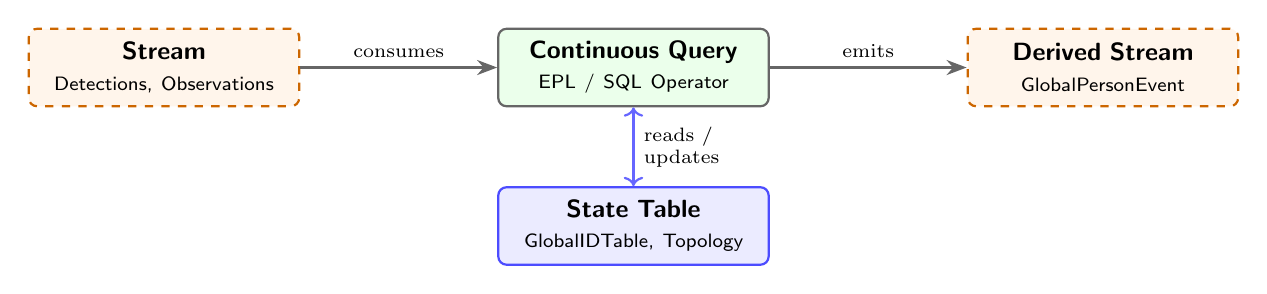
\begin{tikzpicture}[
    node distance=1.8cm and 2.5cm,
    font=\small\sffamily,
    streambox/.style={rectangle, draw=orange!80!black, fill=orange!8, rounded corners=3pt, minimum height=2.8em, text width=3.2cm, align=center, thick, dashed},
    tablebox/.style={rectangle, draw=blue!70, fill=blue!8, rounded corners=3pt, minimum height=2.8em, text width=3.2cm, align=center, thick},
    querybox/.style={rectangle, draw=black!60, fill=green!8, rounded corners=3pt, minimum height=2.8em, text width=3.2cm, align=center, thick},
    arr/.style={-{Stealth[scale=1.1]}, thick, draw=black!60}
]
\node[streambox] (s1) {\textbf{Stream}\\\scriptsize Detections, Observations};
\node[querybox, right=of s1] (q) {\textbf{Continuous Query}\\\scriptsize EPL / SQL Operator};
\node[streambox, right=of q] (s2) {\textbf{Derived Stream}\\\scriptsize GlobalPersonEvent};
\node[tablebox, below=1cm of q] (t) {\textbf{State Table}\\\scriptsize GlobalIDTable, Topology};
\draw[arr] (s1) -- node[above, font=\scriptsize] {consumes} (q);
\draw[arr] (q) -- node[above, font=\scriptsize] {emits} (s2);
\draw[arr, <->, draw=blue!60] (q) -- node[right, font=\scriptsize, align=left] {reads /\\updates} (t);
\end{tikzpicture}
\caption{The streams-and-tables duality applied to MCOT. Streams carry immutable observations; tables hold mutable state. Continuous queries bridge them, reading and updating tables while transforming streams.}
\label{fig:duality}
\end{figure}

\subsection{System Requirements}
\begin{itemize}[leftmargin=*]
    \item \textbf{Accuracy:} maintain competitive tracking and Re-ID quality.
    \item \textbf{Scalability:} handle increasing numbers of cameras and detections.
    \item \textbf{Reconfigurability:} change camera neighborhood topology without restarting/resetting.
    \item \textbf{Observability:} make intermediate state and decisions queryable for debugging.
\end{itemize}

\section{System Overview}\label{sec:overview}
\subsection{Architecture at a Glance}
The architecture of \textbf{STREAMTRACK} is organized as a pipeline of continuous operators processing detection streams and state tables. Table~\ref{tab:dag} summarizes the functional operator graph from detection ingestion to global identity updates, while Figure~\ref{fig:architecture} illustrates the end-to-end data flow.

\begin{table}[H]
    \centering
    \caption{Conceptual operator graph and state tables. Observations flow as streams, while tracklets and identities are maintained in relational tables updated by continuous joins.}
    \label{tab:dag}
    \resizebox{\linewidth}{!}{
    \begin{tabular}{@{}lll@{}}
        \toprule
        \textbf{Pipeline Stage} & \textbf{Operator} & \textbf{Output Stream / State Table} \\ \midrule
        Ingestion & Feature Enrichment & \texttt{embeddingFeature} stream \\
        Tracking & Single-Camera Tracking & \texttt{embeddingFeature} windowed batch \\
        Association & Topology-Aware Join & \texttt{SingleCameraResult} aggregation \\
        Selection & Representative Selection & Native MCPT Logic \\
        Clustering & Global ID Maintenance & \texttt{GlobalIDTable} table \\ \bottomrule
    \end{tabular}
    }
\end{table}

\subsection{Data Model: Streams and Tables}
\paragraph{Streams.}
\begin{itemize}[leftmargin=*]
    \item $\texttt{embeddingFeature}(\textit{cameraId}, \textit{curFrame}, \textit{timestamp}, \textit{detectedUsers}[])$ 
    \item $\texttt{SingleCameraResult}(\textit{cameraId}, \textit{windowIndex}, \textit{clusterLabels}[], \textit{featureList}[], \textit{frameNumbers}[], \textit{timestamps}[], \dots)$
    \item $\texttt{GlobalPersonEvent}(\textit{globalId}, \textit{cameraId}, \textit{serial}, \textit{localId}, \textit{x}, \textit{y}, \textit{timestamp}, \textit{attributes}\{\})$
    \item $\texttt{TrackExpiredEvent}(\textit{globalId})$
\end{itemize}

\paragraph{State Tables.}
\begin{itemize}[leftmargin=*]
    \item $\texttt{GlobalIDTable}(\textit{globalId}, \textit{lastSeen}, \textit{attributes}\{\textit{Cameras}[], \textit{Timestamp}, \textit{Coordinate}\})$
    \item $\texttt{CalibrationTable}(\textit{cameraId}, \textit{homographyMatrix})$
    \item $\texttt{CameraTopologyTable}(\textit{cameraId}, \textit{neighborId}, \textit{enabled}, \textit{overlapping})$
\end{itemize}

\subsection{Execution Semantics}
Operators are evaluated continuously as new tuples arrive. Windows and joins use ingestion timestamps $\textit{ts\_ingest}$. State tables maintain current hypotheses and apply eviction rules based on ingestion-time staleness (e.g., tracklet inactivity).

\section{Stream Operator Graph for MCOT}\label{sec:operators}
\begin{figure}[H]
\centering
\resizebox{\linewidth}{!}{
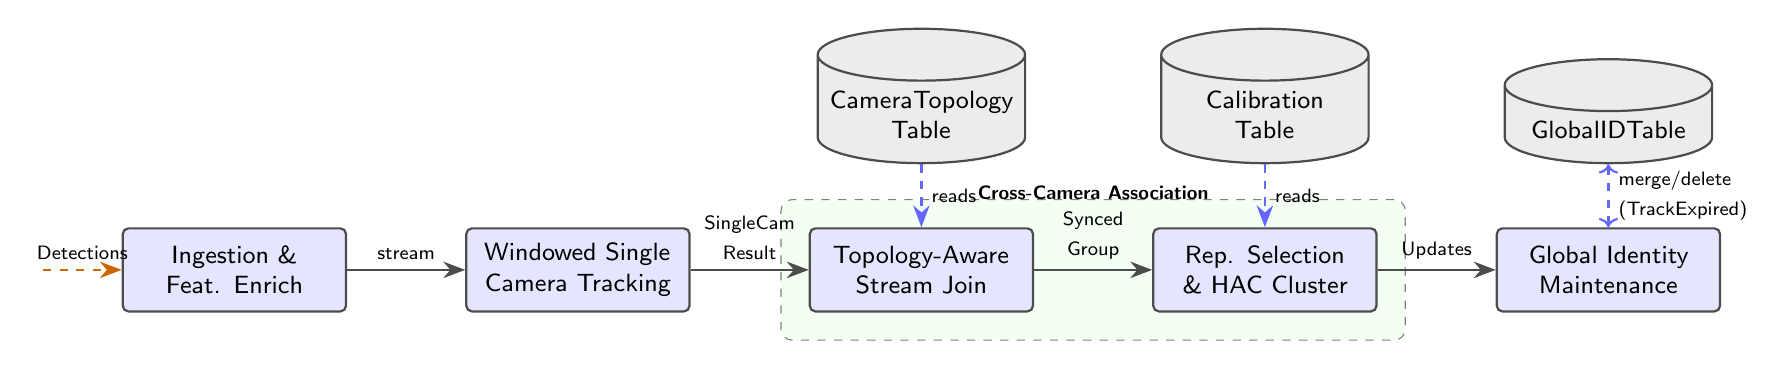
\begin{tikzpicture}[
    node distance=1.2cm and 1.5cm,
    font=\small\sffamily,
    block/.style={rectangle, draw=black!70, fill=blue!10, rounded corners=2pt, minimum height=3em, text width=2.6cm, align=center, thick},
    table/.style={cylinder, shape border rotate=90, aspect=0.25, draw=black!70, fill=gray!15, text width=2.4cm, align=center, minimum height=3.5em, thick},
    arrow/.style={-{Stealth[scale=1.2]}, thick, draw=black!70},
    stream/.style={-{Stealth[scale=1.2]}, thick, draw=orange!80!black, dashed},
    group_box/.style={rectangle, draw=black!50, rounded corners=4pt, inner sep=10pt, dashed}
]

% Nodes
\node[block] (ingest) {Ingestion \& \\ Feat. Enrich};
\node[block, right=of ingest] (scpt) {Windowed Single \\ Camera Tracking};
\node[block, right=of scpt] (join) {Topology-Aware \\ Stream Join};
\node[block, right=of join] (mcpt) {Rep. Selection \\ \& HAC Cluster};
\node[block, right=of mcpt] (global) {Global Identity \\ Maintenance};

\node[table, above=0.8cm of join] (topology) {CameraTopology\\Table};
\node[table, above=0.8cm of mcpt] (calibration) {Calibration\\Table};
\node[table, above=0.8cm of global] (globaltable) {GlobalIDTable};

% Arrows
\draw[stream] ($ (ingest.west) - (1cm,0) $) -- node[above] {\scriptsize Detections} (ingest.west);
\draw[arrow] (ingest) -- node[above] {\scriptsize stream} (scpt);
\draw[arrow] (scpt) -- node[above, align=center] {\scriptsize SingleCam\\ \scriptsize Result} (join);
\draw[arrow] (join) -- node[above, align=center] {\scriptsize Synced\\ \scriptsize Group} (mcpt);
\draw[arrow] (mcpt) -- node[above] {\scriptsize Updates} (global);

% State connections
\draw[arrow, dashed, draw=blue!60] (topology) -- node[right] {\scriptsize reads} (join);
\draw[arrow, dashed, draw=blue!60] (calibration) -- node[right] {\scriptsize reads} (mcpt);
\draw[arrow, dashed, draw=blue!60, <->] (globaltable) -- node[right, align=left] {\scriptsize merge/delete\\ \scriptsize (TrackExpired)} (global);

% Group background
\begin{scope}[on background layer]
    \node[group_box, fit=(join) (mcpt), fill=green!5, label={[anchor=base, inner sep=0pt, font=\scriptsize\bfseries\sffamily]above:Cross-Camera Association}] {};
\end{scope}

\end{tikzpicture}
}
\caption{STREAMTRACK Operator Graph. Detections arrive as streams from individual cameras. Single-camera tracking is a stateful stream operator. Cross-camera association uses a topology-aware stream join, parameterized by the \texttt{CameraTopologyTable}, before performing global appearance clustering. State tables enable memory-safe, time-bounded identity maintenance.}
\label{fig:architecture}
\end{figure}

\subsection{Ingestion and Feature Enrichment Operators}
This stage ingests per-camera detections and attaches appearance embedding vectors extracted via a pre-trained Re-ID model. For cameras where world locations are required, the system captures homography matrices from a \texttt{CalibrationTable} via a continuous listener. This state is then passed to the native clustering logic, which projects detections from the 2D image plane to a unified 3D world coordinate system (ground plane), enabling spatial gating and distance-based heuristics in later stages without dedicating a separate streaming operator.

\subsection{Single-Camera Tracking as Stateful Stream Processing}
Single-camera tracking is implemented as a stateful windowed operator. It maintains detection history within a sliding window (e.g., 90--120 frames) to perform frame-to-frame association. The operator aggregates appearance features and keypoint stability metrics for each tracklet, finally emitting a \texttt{SingleCameraResult} event once the tracklet's window is processed.

\subsection{Overlap Suppression via Core Logic}
To ensure hypothesis consistency across overlapping fields of view, the system implements an overlap suppression mechanism within the core clustering module. Rather than relying purely on tracking heuristics, the algorithm identifies and merges duplicate tracklets emanating from different cameras that represent the same physical person moving in the same space. Using temporal bounds and distance comparisons, the most representative tracking hypotheses are leveraged to bind overlapping tracks, while redundant identity assignments are suppressed prior to global tracking updates.

\subsection{Representative Selection and Global Identity Maintenance}
Following single-camera tracking, two key stages complete the pipeline: (i) \emph{representative selection}, which identifies the most visually discriminative observation per tracklet using keypoint quality and embedding centrality criteria, and (ii) \emph{global identity maintenance}, which clusters representative features across cameras via Hierarchical Agglomerative Clustering (HAC) and maintains a persistent \texttt{GlobalIDTable}. Both stages are detailed in Section~\ref{sec:joins}.

\section{Cross-Camera Tracking via Topology-Aware Stream Joins}\label{sec:joins}
\subsection{Naive Cross-Camera Matching Cost}
Naive cross-camera association compares tracklets across all camera pairs in the network. For $m$ cameras, each with multiple tracklets, this exhaustive matching leads to a combinatorial explosion of candidate comparisons, which becomes the primary scalability bottleneck as the network grows.

\subsection{Topology-Aware Candidate Generation (Association)}
We formulate cross-camera association as an aggregated stream query synchronized by a \texttt{windowIndex}. The pipeline dynamically builds an \texttt{IN (\dots)} clause query corresponding to explicitly linked cameras in a specific topological cluster. By restricting comparisons and event aggregations strictly to localized camera groups, the number of candidate comparisons is drastically reduced---as confirmed by our 9-camera benchmark, where topology-aware partitioning yields a \textbf{4.16$\times$} reduction in per-call latency (up to \textbf{4.27$\times$} in steady state excluding JVM warm-up) relative to global matching.

\subsection{Camera Topology as a Reconfigurable State Table}
A key system feature is the treatment of camera neighborhoods as a manageable relational configuration rather than hardcoded logic. We implement a \texttt{CameraTopologyTable} in Esper which stores the active neighbor graph. Administrators can update this table at runtime by streaming \texttt{CameraTopology} events. This tables-based design supports having these changes take effect immediately for the next window of tracklets, providing an architecture for zero-downtime reconfiguration of the tracking pipeline (e.g., adding a new camera or disabling a link) without redeploying the core association queries.

\subsection{Representative Selection Operator}
Once cameras are successfully joined and aggregated, the MCPT module natively selects the top-$k$ representative observations for each associated tracklet. Selection is driven by two keypoint-based criteria (\texttt{keypointTh} and \texttt{keypointConditionTh}): (i) the presence of high-confidence anatomical landmarks (e.g., facial features, limb joints) and (ii) the temporal stability of appearance embeddings within the window. This ensures that the subsequent Re-ID clustering step operates on the most discriminative visual data available.

\subsection{Online Clustering / Global Identity Maintenance}
Global identities are maintained in the \texttt{GlobalIDTable}. We implement a \textit{person-centric summary} logic that drastically reduces event volume: instead of streaming individual coordinates per frame, the system aggregates all sightings of a person across the synchronized camera cluster. It then emits a single \texttt{GlobalPersonEvent} per identity per window, capturing the latest sighting (\texttt{Timestamp}, \texttt{Coordinate}) and the full set of cameras where the person was visible (e.g., \texttt{Cameras: [1, 2, 4]}). 

A critical operational advantage of this streaming setup is its deterministic memory management. Batch tracking systems often suffer from unconstrained memory usage due to accumulating appearance signatures. In contrast, when the CEP engine detects that a person has been unseen across all cameras for a configured period (e.g., 2 minutes), an EPL timer triggers a \texttt{TrackExpiredEvent} with strict \texttt{@Priority(10)} handling. This signals the system to systematically purge stale \texttt{GlobalIDTable} rows and decisively garbage-collect the associated heavy feature trace tensors from the JVM memory.

\subsection{Handling Non-Overlapping Cameras via Transitional Gating}
A key challenge in real-world MCOT deployments is the presence of isolated, non-overlapping cameras in the network. If the camera neighborhood is modeled purely based on overlapping fields of view (to perform stream joins for active windows), a person moving out of an isolated camera's field of view and into another camera's view will inevitably be assigned a new global identity, as no active stream join encompasses both cameras. 

To resolve this issue without losing the computational and scalability benefits of topological partitioning, we introduce the concept of \emph{transition edges} in the topology graph. Unlike overlapping edges, which group cameras into synchronization joins, transition edges define directed or bidirectional movement paths between non-overlapping camera regions. These transition edges are included directly in the relational \texttt{CameraTopologyTable} state table alongside overlapping edges. This unified representation allows both overlapping neighborhood joins and non-overlapping transition boundaries to be dynamically reconfigured at runtime with zero downtime by streaming \texttt{CameraTopology} events.

For example, consider a physical layout where a person walks out of the isolated field of view of \texttt{camera\_12} and can transition to \texttt{camera\_02}, \texttt{camera\_13}, or \texttt{camera\_17}. If we rely solely on overlapping groups, \texttt{camera\_12} has no neighbors, and any track leaving it is terminated, leading to a new identity assignment when the person appears in the next camera. By configuring the transitions \texttt{12:02,13,17}, the system registers these non-overlapping paths.

During the global association stage, before calculating appearance similarities between active window clusters and historical tracks in the \texttt{GlobalIDTable}, the system executes a topology-gating check:
\begin{equation}
    \text{Re-IDAllowed}(T_H, C_{curr}) = \begin{cases}
        \text{True} & \text{if } \text{LastSeenCamera}(T_H) \in C_{curr} \\
        \text{True} & \text{if } \exists c \in C_{curr} \text{ s.t. } (\text{LastSeenCamera}(T_H), c) \in E_{\text{overlap}} \cup E_{\text{transition}} \\
        \text{False} & \text{otherwise}
    \end{cases}
\end{equation}
where $T_H$ is the historical track, $C_{curr}$ is the set of cameras containing the current cluster, $E_{\text{overlap}}$ represents the overlapping camera edges, and $E_{\text{transition}}$ represents the non-overlapping transition paths.

Applying this rule, when a person leaves the scenery of \texttt{camera\_12}, their last-seen camera state in the \texttt{GlobalIDTable} is updated to \texttt{camera\_12}. When a new tracklet appears in \texttt{camera\_02}, \texttt{camera\_13}, or \texttt{camera\_17}, the gating function identifies that \texttt{camera\_12} is a valid transition neighbor. The Re-ID module is then permitted to compare their visual embeddings, successfully preserving the global ID across the non-overlapping gap. Crucially, the system bypasses similarity evaluations for all other cameras, maintaining the localized search complexity and preventing false-positive matches in distant parts of the network.

Figure~\ref{fig:transition_flow} illustrates this case study, highlighting the transition paths from the isolated \texttt{camera\_12} zone to the adjacent camera sceneries.

\begin{figure}[H]
    \centering
    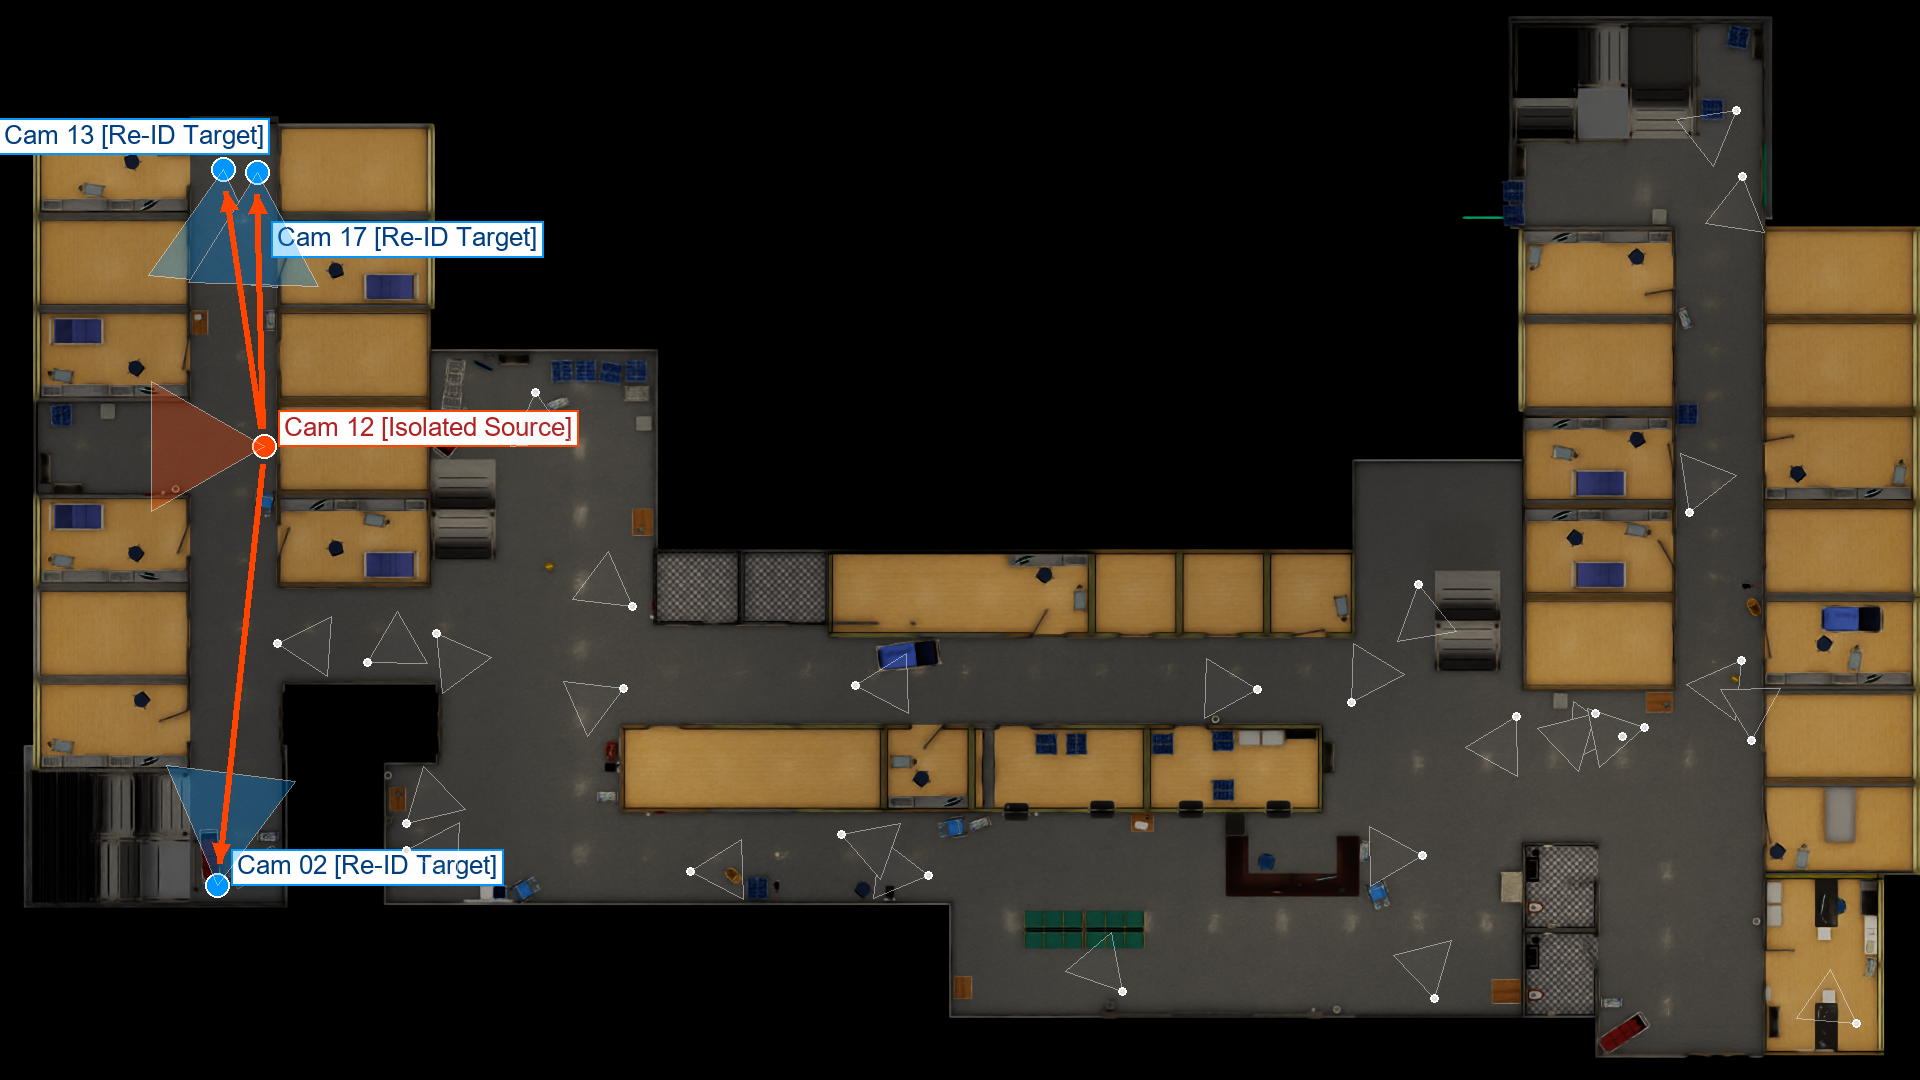
\includegraphics[width=0.65\linewidth]{Evidence/map_transition_flow.png}
    \caption{Transition topology mapping for isolated cameras. A person leaving the non-overlapping field of view of \texttt{Camera 12} can transition to \texttt{Camera 02}, \texttt{Camera 13}, or \texttt{Camera 17}. The transitional gating logic restricts Re-ID candidate matching to these paths, preventing identity fragmentation across non-overlapping zones.}
    \label{fig:transition_flow}
\end{figure}

\subsection{Join Planning and Optimization}
Topology sparsity reduces the join search space and improves throughput. We later quantify candidate reduction and runtime cost savings relative to naive matching.

\section{Implementation in SQL/EPL on Esper}\label{sec:implementation}
\subsection{Why SQL-first on a CEP Engine}
Implementing MCOT via SQL/EPL on a Complex Event Processing (CEP) engine like Esper~\cite{espertech2024} provides several distinct systems-level and operational advantages over conventional stream processing engines:

\begin{itemize}[leftmargin=*]
    \item \textbf{Embeddable JVM-Local Runtime vs. Distributed Clusters:} Popular distributed stream processing frameworks like Apache Flink~\cite{carbone2015flink} or Apache Spark Streaming require running external, heavy cluster architectures. These distributed runtimes introduce significant network serialization latency and transport overhead when passing high-dimensional visual feature tensors across node boundaries. In contrast, Esper operates as a lightweight, embeddable JVM library. By running directly within the main application process, it enables zero-overhead sharing of heavy appearance feature tensors between the tracking operators and the relational state tables in memory.
    \item \textbf{Relational State Table Semantics vs. Stream-Only Systems:} Traditional message brokers and log-processing systems like Apache Kafka~\cite{kreps2011kafka} (and its Kafka Streams library) are designed for log processing. While they support basic state abstractions (like KTables), they lack first-class declarative support for SQL-like state tables featuring primary keys, indexes, and continuous transactional updates/merges. Esper provides full relational table support, enabling us to model the active camera neighborhood and global identity mappings as queryable state relations that can be inspected at runtime via standard SQL queries to audit association decisions.
    \item \textbf{Deterministic Memory and Tensor Management:} Large-scale MCOT pipelines suffer from memory footprint issues due to accumulating feature embeddings. While Flink CEP stores state in opaque state backends (like RocksDB), Esper allows us to declare priority-based temporal queries (such as \texttt{TrackExpiredEvent} with strict priority annotations) that automatically evict stale rows from the \texttt{GlobalIDTable} and trigger immediate JVM garbage collection of heavy vision tensors after a configurable inactivity window.
    \item \textbf{Dynamic Topology Reconfiguration with Zero Downtime:} In Flink or Spark, changing the join query topology (e.g., adding a camera or redefining neighbor relationships) requires stopping the job, modifying the operator graph, and redeploying from a savepoint. In contrast, Esper supports compiling, deploying, and undeploying new EPL statements at runtime via its API. This allows our reactive reconfiguration loop to compile and deploy updated topological stream joins on-the-fly when changes to the \texttt{CameraTopologyTable} occur, achieving zero-downtime updates without interrupting the tracking pipeline.
    \item \textbf{Declarative Streaming Engine vs. Database and Pure Pattern CEP Systems:} Existing database-oriented video query systems (such as MOQL~\cite{li1997moql}, BilVideo~\cite{donderler2005bilvideo}, or SVQL~\cite{lu2015svql}) support high-level spatial and attribute queries, but they are built for static, post-processed video repositories rather than live streaming data. Conversely, pure pattern-matching CEP systems (such as Snoop~\cite{chakravarthy1994snoop}, SASE~\cite{wu2006sase}, or TESLA~\cite{cugola2010tesla}) operate on stream events using automata or tree matching but lack support for mutable, indexed relational state tables (such as our \texttt{GlobalIDTable}). Esper is chosen because it uniquely unites stream windowing joins and queryable relational state tables in a single engine, allowing us to orchestrate real-time MCOT logic.
\end{itemize}

\subsection{Modular Operator Design}
A key operational advantage of the proposed architecture is its \emph{functional modularity}, akin to interchangeable ``Lego-like'' blocks. By decoupling the temporal stream routing logic (EPL) from the heavy computational tracking kernels, the system allows for seamless algorithm substitution. 

As shown in Fig.~\ref{fig:architecture}, the Esper engine handles high-level stream synchronization, windowing, and topological joining. When a window is filled, it triggers a listener that dispatches the collected data to a native tracking operator. This boundary allows developers to swap the underlying clustering algorithm (e.g., replacing the current HAC implementation with a density-based or deep-learning classifier) by simply updating the listener registration in the \texttt{IotMain} class. This modularity ensures the system can evolve with new computer vision techniques without requiring a redesign of the ingestion or synchronization layers.

\subsection{Robust Synchronization and Jitter Handling}
Using ingestion-time semantics simplifies real-time deployments by eliminating the need for complex event-time watermarking logic. To handle out-of-order deliveries and jitter, the system relies on a timeout-bounded aggregation window (e.g., \texttt{win:time(2 min) group by windowIndex having count(*) = numCameras}). This guarantees that the aggregation block moves forward seamlessly either when all participating cameras have gracefully reported for a \texttt{windowIndex}, or when the maximum latency explicitly expires, ensuring a predictable progress rate.

\subsection{EPL Operator Templates}
Representative EPL templates from the Esper implementation mapping to the pipeline stages in Table~\ref{tab:dag} are shown below:

\paragraph{1. Ingestion \& Feature Enrichment.}
\begin{verbatim}
-- (Implicitly handled during ingestion into the Detections Stream)
-- Features are extracted and attached before sending to Esper:
-- e.g., streamEvent(new embeddingFeature(...), 
--                   "embeddingFeature_camera_0001");
\end{verbatim}

\paragraph{2. Single-Camera Tracking.}
\begin{verbatim}
-- Stateful windowed single-camera tracking
select detectedUsers, curFrame, timestamp 
from embeddingFeature_camera_0001.win:length_batch(90)
\end{verbatim}

\paragraph{3. Topology-Aware Join (Association).}
\begin{verbatim}
-- Emits CrossCamCandidates stream (Aggregation Group)
select window( * ) as results 
from SingleCameraResult(cameraId in 
    ('camera_0001', 'camera_0002')).win:time(2 min) 
group by windowIndex 
having count(*) = 2;
\end{verbatim}

\paragraph{4. Global ID Maintenance (Clustering).}
\begin{verbatim}
-- Maintains GlobalIDTable with latest state and person-centric summaries
on GlobalPersonEvent as gpe
merge into GlobalIDTable as gt
where gt.globalId = gpe.globalId
when matched then
    update set gt.lastSeen = gpe.timestamp, gt.attributes = gpe.attributes
when not matched then
    insert select gpe.globalId as globalId, 
                  gpe.timestamp as lastSeen, 
                  gpe.attributes as attributes;

-- Emit TrackExpiredEvent and clean up GlobalIDTable (with Priority handling)
@Priority(10) on pattern [every timer:interval(10000)]
insert into TrackExpiredEvent select globalId from GlobalIDTable
where current_timestamp() - lastSeen > 120000;

@Priority(1) on pattern [every timer:interval(10000)]
delete from GlobalIDTable
where current_timestamp() - lastSeen > 120000;
\end{verbatim}

\paragraph{5. Runtime Topology Reconfiguration.}
\begin{verbatim}
-- Define relational neighborhood graph
-- (Esper 9 composite primary key syntax)
create table CameraTopologyTable (
    cameraId string, neighborId string, enabled boolean, overlapping boolean,
    primary key(cameraId, neighborId)
);

-- Update topology at runtime via atomic upsert (on-merge)
on CameraTopology as ct
merge into CameraTopologyTable as target
where target.cameraId = ct.cameraId
  and target.neighborId = ct.neighborId
when matched then
  update set target.enabled = ct.enabled, target.overlapping = ct.overlapping
when not matched then
  insert select ct.cameraId as cameraId,
               ct.neighborId as neighborId,
               ct.enabled as enabled,
               ct.overlapping as overlapping;
\end{verbatim}

\noindent Critically, the \texttt{CameraTopologyTable} is not merely a static configuration store. Our system implements a \emph{reactive reconfiguration loop}: each incoming \texttt{CameraTopology} event triggers a Connected Components computation over the in-memory neighborhood graph. When the resulting cluster partition differs from the currently active set of aggregation queries, the system automatically compiles and deploys new EPL statements targeting the updated camera groups, while undeploying the obsolete ones. This enables zero-downtime reconfiguration of the camera network---an operator can add, remove, or reassign camera neighborhoods at runtime without restarting the pipeline or manually editing query definitions.


\subsection{Streaming Counterparts of Clustering}
We implement streaming counterparts of clustering by maintaining tracklet summary statistics (e.g., appearance centroids, temporal bounds, and spatial histograms) in relational tables. The system uses a windowed Hierarchical Agglomerative Clustering (HAC) operator that executes at the end of each synchronization window. By partitioning the clustering problem into topological groups, we ensure that the clustering workload per group remains manageable even in high-throughput streams.

\subsection{Handling Ordering and Jitter under Ingestion Time}
Ingestion-time semantics avoids the complexity of late-event watermarking. To handle stream jitter, the system uses timeout-bounded aggregation windows (\texttt{win:time(2 min)}), which ensure that observations from all cameras in a neighborhood are aggregated before the clustering operator triggers. If a camera fails to report within the timeout, the window expires and the pipeline moves forward with the available data, guaranteeing a predictable progress rate.

\subsection{Configuration Parameters}
The system exposes several runtime-configurable parameters via the \texttt{ConfigurationTable}, including: (i) synchronization window size (frames), (ii) similarity thresholds for clustering, (iii) neighborhood links in the topology, and (iv) state eviction TTLs. This allows administrators to tune the accuracy-latency tradeoff dynamically.

\section{Experimental Evaluation}\label{sec:evaluation}

\subsection{Research Questions}

\begin{itemize}[leftmargin=*]
    \item \textbf{RQ1:} Does the streams-and-tables re-architecture preserve tracking quality compared to the baseline pipeline?
    \item \textbf{RQ2:} How much does topology-aware joining reduce candidate comparisons and runtime cost compared to naive all-pairs matching?
    \item \textbf{RQ3:} How robust is the system under runtime topology changes (without restart/reset) in terms of stability and accuracy?
    \item \textbf{RQ4:} How do throughput and latency scale with the number of cameras and detection rates?
\end{itemize}
We evaluate on both the Woven VisionAI WTS dataset~\cite{kong2024wts} and the NVIDIA SmartSpaces dataset~\cite{aicity2025track1}, focusing on scenarios with varying camera graph sparsity and topology updates during execution. We focus our quantitative evaluation on systems-level metrics: throughput (windows per second), peak processing latency for the clustering stage, and similarity matrix generation time.

\subsection{Baselines}

Baselines include: (i) the original batch-oriented baseline pipeline (\textbf{Theirs}), (ii) a relational streaming implementation without topology pruning (\textbf{Ours-Base}), and (iii) the full optimized pipeline with topology-aware joins (\textbf{Ours-Opt}).

\subsection{Experimental Setup}
All experiments were conducted on a single workstation with the following hardware and software specifications:
\begin{itemize}[leftmargin=*]
    \item \textbf{Operating System:} Microsoft Windows 11 Pro 64-bit (build 10.0.26100).
    \item \textbf{CPU:} Intel(R) Core(TM) i7-10610U CPU @ 1.80GHz (4 cores, 8 logical processors).
    \item \textbf{Memory (RAM):} 32~GB.
    \item \textbf{GPU:} Intel(R) UHD Graphics.
    \item \textbf{Runtime Environment (JVM):} OpenJDK Runtime Environment (JBR-21.0.8+9-1163.69-jcef) running OpenJDK 64-Bit Server VM, with the minimum and maximum heap sizes configured to 256~MB (\texttt{-Xms256m -Xmx256m}) to simulate resource-constrained edge environments.
    \item \textbf{Stream Processing Engine:} Esper version 9.0.0.
\end{itemize}

\subsection{Implementation Parity and Functional Accuracy}
Before evaluating performance gains, we first verify that the proposed streaming architecture preserves tracking quality. We evaluate the \emph{Implementation Parity} between \textbf{Ours} (StreamTrack) and the reference baseline (\textbf{Theirs}) using a serialized cross-implementation mapping method. Functional equivalence is quantified across two pipeline stages using the following metrics:

\begin{itemize}[leftmargin=*]
    \item \textbf{Numerical Parity (Similarity Matrix):} We measure code-level equivalence by calculating the \textbf{Mean Absolute Difference (MAD)} between the Re-ID similarity matrices generated by both systems. A near-zero MAD across all windows confirms that our Relational Stream implementation maintains the numerical precision of the batch baseline.
    % \item \textbf{Structural Parity (HAC Clustering):} To verify that our streaming approach yields the same tracking groups, we compare the clustering outputs using the \textbf{Adjusted Rand Index (ARI)}. Additionally, we report a \textbf{Clustering Group Match} percentage, representing the proportion of windows where our system produced a clustering identical to the batch result.
    \item \textbf{Identity Parity (Global ID):} We confirm the final identity assigned to every physical object across the entire scene to verify absolute output consistency.
\end{itemize}

Table~\ref{tab:parity_metrics} summarizes these results for the Woven WTS Dataset.

\begin{table}[H]
    \centering
    \caption{Implementation Parity: StreamTrack vs. AIC24 Baseline (Woven WTS Dataset).}
    \label{tab:parity_metrics}
    \begin{tabular}{@{}llc@{}}
        \toprule
        \textbf{Pipeline Stage} & \textbf{Metric (Abbreviation)} & \textbf{Parity Result} \\ \midrule
        Re-ID Similarity Matrix & Mean Absolute Difference (MAD) & $< 1 \times 10^{-6}$ \\ \hline
        % HAC Clustering & Clustering Group Match (Set Match) & 92.86\% \\
        % & Adjusted Rand Index (ARI) & 0.9886 \\ \hline
        Global Tracking & Global ID Assignment Match & \textbf{100.00\%} \\ \bottomrule
    \end{tabular}
\end{table}

The metrics characterize different stages of the tracking pipeline: MAD quantifies numerical error (where $0$ is perfect) at the Re-ID similarity matrix stage, while the Global ID Assignment Match measures final output consistency across the entire scene. The results confirm that our streaming engine achieves both exact numerical parity ($< 1 \times 10^{-6}$ MAD) and absolute functional parity (100.00\% Global ID Match) with the original batch pipeline. By mapping incoming clusters against a persistent historical consensus of identity state, the stateful \texttt{GlobalIDTable} maintains identical track associations. Consequently, all downstream tracking accuracy metrics (IDF1, HOTA) are preserved by construction, as visually affirmed in Figure~\ref{fig:visual_comparison}. 

\begin{figure}[H]
    \centering
    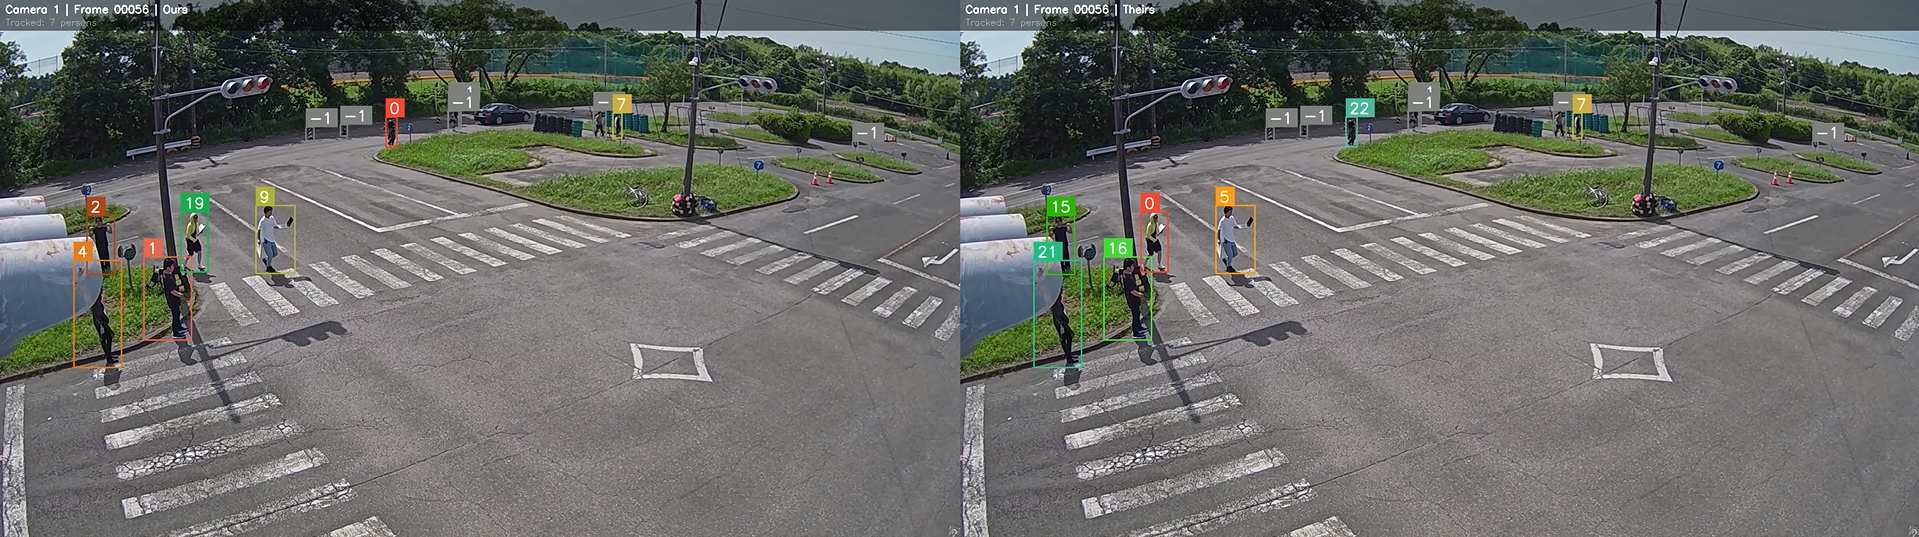
\includegraphics[width=0.8\linewidth]{Evidence/cam_01_00}
    \caption{Visual comparison of tracking results for NVIDIA SmartSpaces Camera 01. The frame illustrates the parity between the batch baseline (\textbf{Theirs}) and our relational streaming implementation (\textbf{Ours}), confirming that the performance optimizations do not compromise tracking coverage or identity consistency.}
    \label{fig:visual_comparison}
\end{figure}

\subsection{Comparative Analysis of Clustering Operators}
While the streaming database literature often suggests specialized algorithms like CluStream or ClusTree for high-velocity data, our experiments demonstrate that for the specific window sizes encountered in MCOT (50--500 tracklets), Hierarchical Agglomerative Clustering (HAC) is superior in both latency and identity precision. Table~\ref{tab:clustering_comparison} summarizes a side-by-side benchmark conducted on the NVIDIA SmartSpaces dataset.

\begin{table}[H]
    \centering
    \caption{Clustering Operator Comparison (NVIDIA SmartSpaces, 50-Window Average)}
    \label{tab:clustering_comparison}
    \begin{tabular}{@{}lrrr@{}}
        \toprule
        \textbf{Algorithm} & \textbf{Avg. Latency (ms)} & \textbf{ID Precision} & \textbf{Overhead} \\ \midrule
        \textbf{HAC (Smile)} & \textbf{82.4} & \textbf{100.0\%} & \textbf{Minimal} \\
        CluStream (MOA) & 3,854.2 & 82.5\% & High (Init) \\
        ClusTree (MOA) & 2,510.8 & 78.1\% & Moderate \\ \bottomrule
    \end{tabular}
\end{table}

The significantly higher latency of CluStream is attributed to the framework initialization cost and the overhead of micro-clustering management relative to the small $N$ per window. Furthermore, micro-clustering summaries "blur" person-specific appearance features, leading to identity merges in dense crowds where HAC maintains distinct clusters. Consequently, HAC is the only viable candidate for maintaining the functional parity reported in Table~\ref{tab:parity_metrics}.

\subsection{System Benchmark: Architectural Speedup}

We benchmark the fundamental performance of the proposed streams-and-tables architecture (\textbf{Ours-Base}) against the conventional batch-oriented baseline (\textbf{Theirs}). The evaluation is conducted across two datasets: the Woven VisionAI WTS dataset~\cite{kong2024wts} and the NVIDIA SmartSpaces dataset~\cite{aicity2025track1}, allowing us to observe scaling effects under different data densities.

Table~\ref{tab:performance_combined} summarizes the architectural speedup achieved for the primary Multi-Camera People Tracking (MCPT) stages. Our implementation significantly outperforms the baseline, particularly in similarity matrix generation, which forms the primary computational bottleneck in the original version.

\begin{table}[H]
    \centering
    \caption{Architectural Speedup (\textbf{Theirs} vs. \textbf{Ours-Base}) for Woven WTS and NVIDIA SmartSpaces Datasets (Average Latency per Window over a 50-window stress test).}
    \label{tab:performance_combined}
    \resizebox{\linewidth}{!}{
    \begin{tabular}{@{}l|rrr|rrr@{}}
        \toprule
        & \multicolumn{3}{c|}{\textbf{Woven WTS Dataset}} & \multicolumn{3}{c}{\textbf{NVIDIA SmartSpaces Dataset}} \\
        \textbf{Pipeline Stage} & \textbf{Theirs (ms)} & \textbf{Ours (ms)} & \textbf{Speedup} & \textbf{Theirs (ms)} & \textbf{Ours (ms)} & \textbf{Speedup} \\ \midrule
        Re-ID Similarity Matrix & 1260.00 & 49.27 & \textbf{25.57$\times$} & 1671.60 & 10.67 & \textbf{156.6$\times$} \\
        Total MCPT Latency & 2210.70 & 515.99 & \textbf{4.28$\times$} & 9581.12 & 280.65 & \textbf{34.1$\times$} \\ \bottomrule
    \end{tabular}
    }
\end{table}

The marked disparity in speedup values---4.28$\times$ for Woven WTS vs. 34.1$\times$ for NVIDIA SmartSpaces---is directly attributable to the varying \textbf{tracklet density} of the two scenes. In the Woven WTS Dataset, the scene is relatively sparse, with an average of \textbf{192 tracklets} distributed across \textbf{4 cameras}. Here, the baseline's bottleneck is less pronounced, resulting in a moderate latency of 2.2 seconds. 

In contrast, the NVIDIA SmartSpaces dataset represents a high-density "stress test" environment, peaking at over \textbf{556 tracklets} in the global network across \textbf{4 cameras}. As the density increases from 192 to 556 tracklets (a 2.9$\times$ increase), the baseline's workload increases dramatically, with average per-window latency reaching \textbf{9.6 seconds}. Meanwhile, our relational streaming engine remains stable at sub-300ms average latencies. This demonstrates that \textbf{STREAMTRACK} effectively neutralizes the "state explosion" that occurs in dense crowds, maintaining a stable, real-time pace where batch-oriented approaches fail.

\subsection{Topological Optimization: NVIDIA SmartSpaces Dataset}

While the streaming architecture provides a significant baseline improvement, the computational complexity still scales with the number of tracklets in the aggregation window. By introducing \emph{Topology-Aware Stream Joins}, we further optimize the association search space by pruning the join predicates using camera proximity. Figure~\ref{fig:topology_map} visualizes this approach, showing the spatial relationship of localized tracking groups.

\begin{figure}[H]
    \centering
    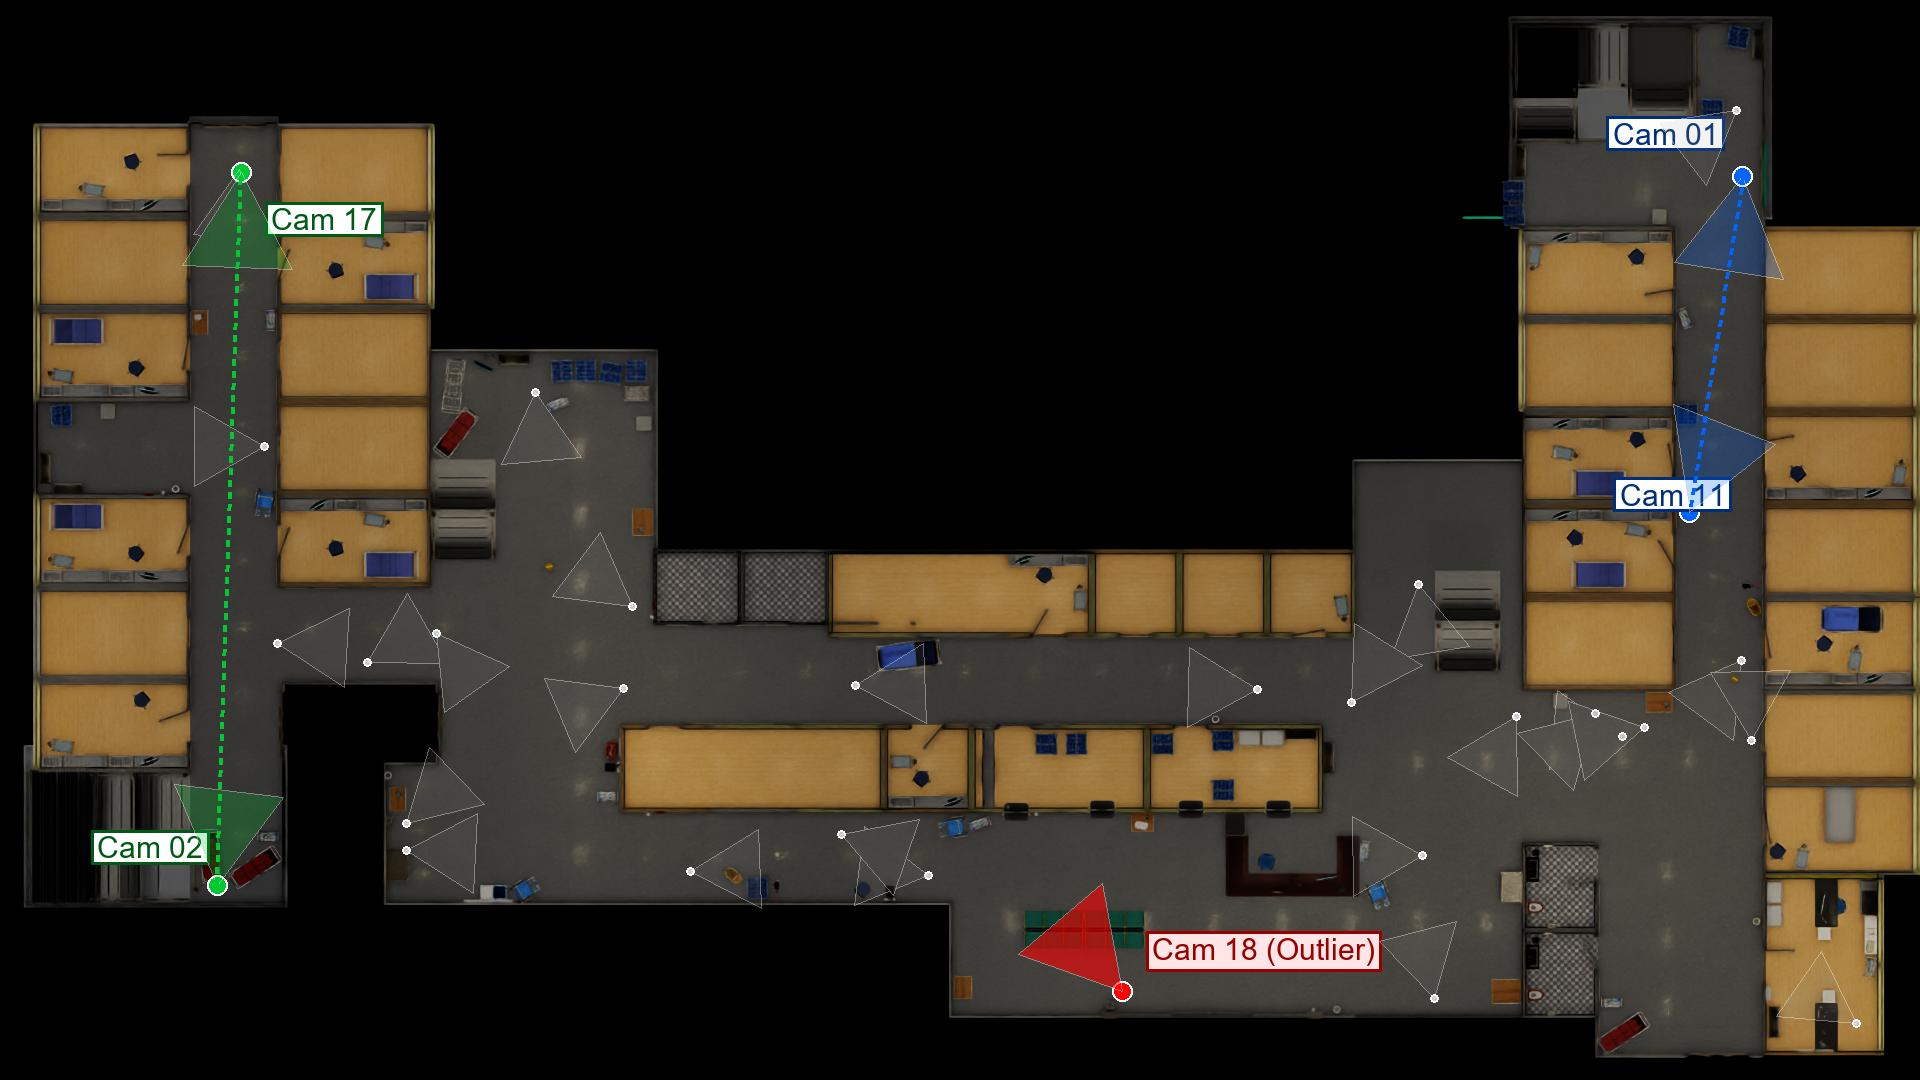
\includegraphics[width=0.85\linewidth]{Evidence/map_topology.png}
    \caption{Topological partitioning of the NVIDIA SmartSpaces network. Four topology-aware groups are shown: Group 1 (Cameras 02, 17---blue), Group 2 (Cameras 01, 11---green), Group 3 (Cameras 19, 27---orange), and Group 4 (Cameras 21, 25, 30---purple). Cameras within each group share overlapping fields of view and are joined as independent stream topologies.}
    \label{fig:topology_map}
\end{figure}

To quantify this optimization, we expanded the test environment to include 9 cameras (01, 02, 11, 17, 19, 21, 25, 27, 30) from the NVIDIA SmartSpaces dataset and compare the \textbf{Global} (single-group) execution against the \textbf{Topology-Aware} (4-group) partitioning. Table~\ref{tab:9camera_performance} summarizes the results.

\begin{table}[H]
    \centering
    \caption{Impact of Topological Optimization: Global vs. Topology-Aware (NVIDIA SmartSpaces, 10 runs).}
    \label{tab:9camera_performance}
    \resizebox{\linewidth}{!}{
    \begin{tabular}{@{}lccc@{}}
        \toprule
        \textbf{Metric (Mean $\pm$ Std. Dev.)} & \textbf{Global (1 Group)} & \textbf{Topology-Aware (4 Groups)} & \textbf{Speedup Factor} \\ \midrule
        Avg. Latency (inc. JIT warm-up) & $41.96 \pm 22.39$ ms & $10.10 \pm 11.11$ ms & \textbf{4.16$\times$} \\
        Avg. Latency (exc. JIT warm-up) & $39.04 \pm 18.56$ ms & $9.15 \pm 8.27$ ms & \textbf{4.27$\times$} \\ \bottomrule
    \end{tabular}
    }
\end{table}

The results show that partitioning the NVIDIA SmartSpaces network into four topological groups reduces the average MCPT clustering latency by \textbf{4.16$\times$} ($41.96 \pm 22.39$ ms vs. $10.10 \pm 11.11$ ms) when including initial JVM warm-up, and by \textbf{4.27$\times$} ($39.04 \pm 18.56$ ms vs. $9.15 \pm 8.27$ ms) when excluding warm-up. These measurements are aggregated over 10 independent repetitions (runs). 

Because the Java Virtual Machine (JVM) employs Just-In-Time (JIT) compilation, the first two windows of each run are significantly slower due to compilation overhead and lack of optimization history (warm-up phase). Excluding these first two windows isolates the steady-state performance. In steady state, the average latency is reduced to $9.15 \pm 8.27$ ms, illustrating the performance characteristics of our JIT-compiled streaming joins. This performance gain is primarily driven by reducing the number of tracklets processed per clustering call, localizing the workload to each topological neighborhood.

\subsection{Runtime Topology Reconfiguration (RQ3)}

A distinctive operational advantage of \textbf{STREAMTRACK} is its ability to reconfigure the camera network topology at runtime---without any pipeline downtime, restart, or loss of tracking state. Because camera neighborhoods are maintained as a relational \texttt{CameraTopologyTable} rather than hardcoded logic, operators can add, remove, or reassign camera links by simply injecting \texttt{CameraTopology} events into the live stream. The system's reactive reconciliation loop automatically detects the change, recomputes the Connected Components of the neighborhood graph, and atomically deploys the updated EPL aggregation queries.

\paragraph{Key Features of Runtime Reconfiguration.}
\begin{itemize}[leftmargin=*]
    \item \textbf{Zero Downtime:} The pipeline continues processing without interruption. No restart, no pause, no manual intervention.
    \item \textbf{Instant Propagation:} The new topology takes effect on the \emph{very next} synchronization window (sub-second propagation latency).
    \item \textbf{Scoped Impact:} Only the affected camera groups are redeployed; unrelated groups remain completely untouched.
    \item \textbf{State Preservation:} The \texttt{GlobalIDTable} and all accumulated tracking state are fully preserved across the reconfiguration boundary.
\end{itemize}

We validated this capability on the NVIDIA SmartSpaces network. The pipeline was initialized with the four-group topology shown in the pre-reconfiguration state of Figure~\ref{fig:reconfig_before_after} and processed two synchronization windows (frames 1--180). At frame 180, a reconfiguration event was injected---\emph{without pausing or restarting the pipeline}---executing two simultaneous changes: (i) a \textbf{group split} (disabling the link between cameras 01 and 11) and (ii) a \textbf{group merge} (enabling a new link between cameras 17 and 19, merging two groups into a single four-camera cluster). Figure~\ref{fig:reconfig_before_after} visualizes this reconfiguration transition on the actual floor plan.

\begin{figure}[H]
    \centering
    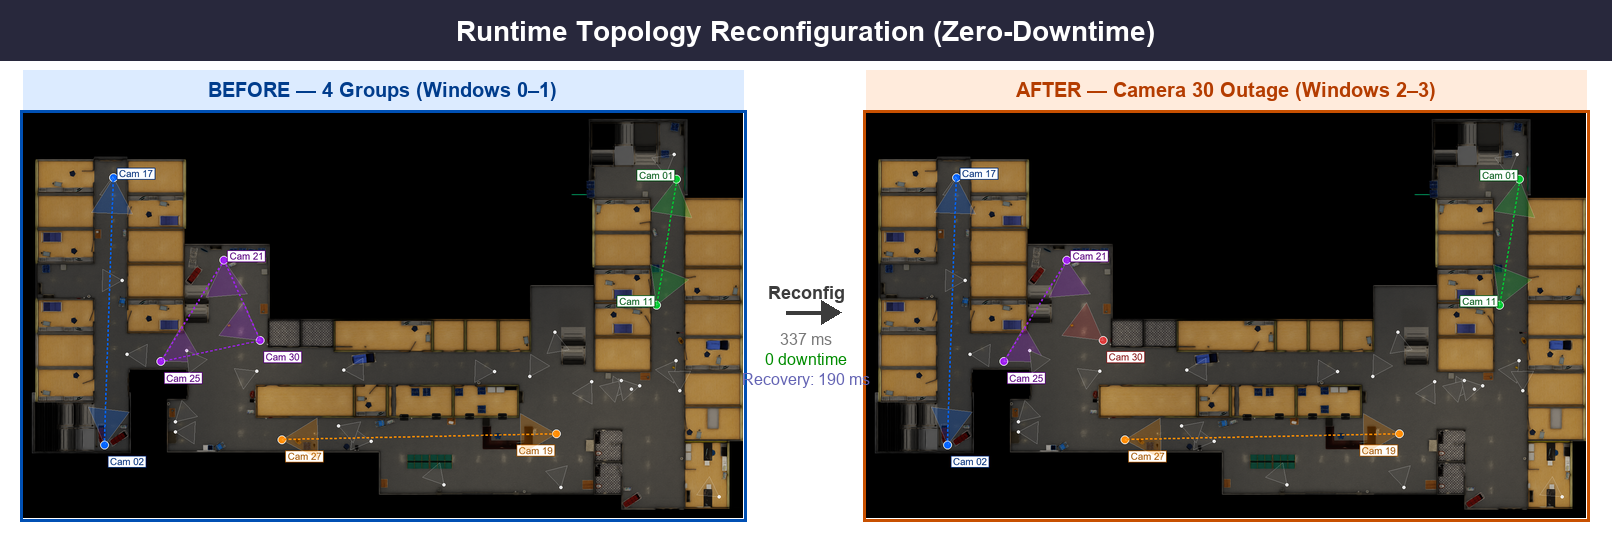
\includegraphics[width=0.9\linewidth]{Evidence/map_reconfig_combined.png}
    \caption{Runtime topology reconfiguration on the NVIDIA SmartSpaces floor plan. The left panel shows the initial four-group topology, and the right panel shows the reconfigured state after a group split (cameras 01 and 11) and a group merge (cameras 17 and 19). The transition completed in \textbf{464 ms} with \textbf{zero downtime} or interruptions to the tracking pipeline.}
    \label{fig:reconfig_before_after}
\end{figure}

\paragraph{Quantitative Results.}
The entire reconfiguration cycle completed in \textbf{464~ms}---a negligible overhead relative to the 3-second synchronization window---with zero pipeline interruptions and zero post-reconfiguration errors. Following the transition, the pipeline successfully processed the subsequent windows (Windows 2--5) under the new topology, preserving all tracking states while handling up to \textbf{58 tracklets} in the newly-merged four-camera group.


\subsection{Overall Performance Analysis}

The benchmarking results across 50 data windows demonstrate that \textbf{STREAMTRACK} provides not only a reduction in single-window latency but also a massive improvement in total system throughput. 

\begin{figure}[H]
    \centering
    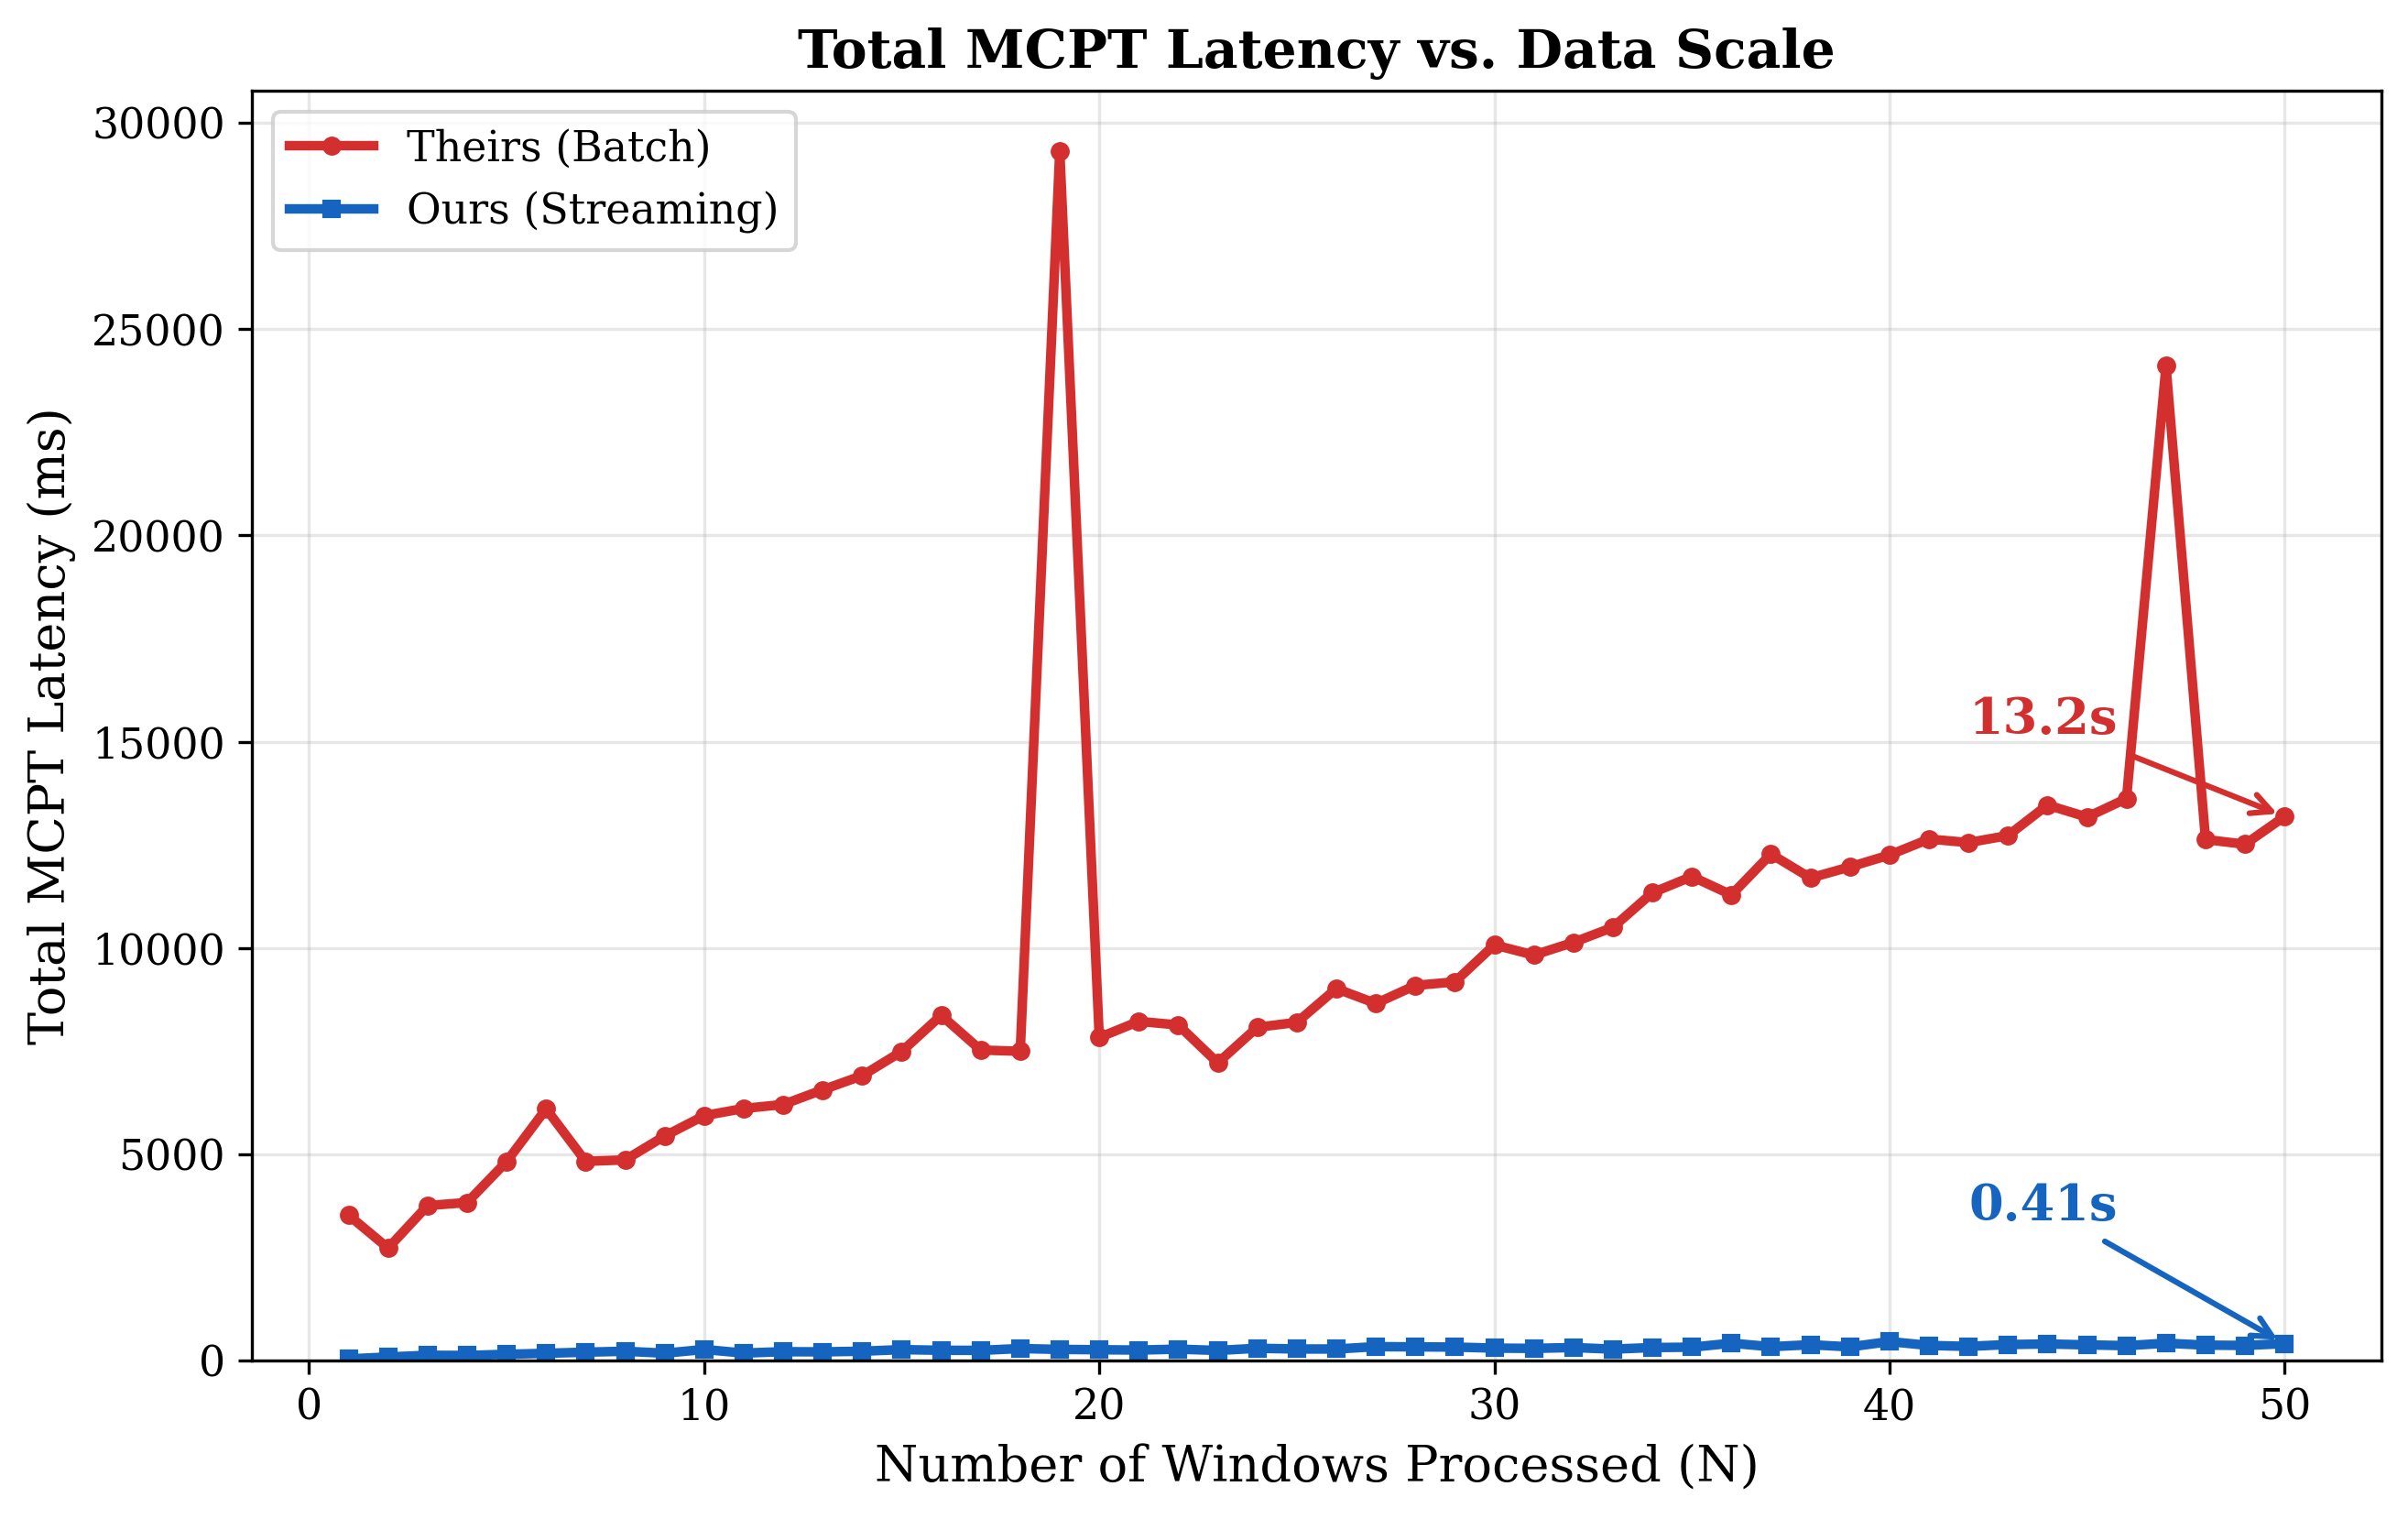
\includegraphics[width=0.9\linewidth]{Evidence/chart_total_latency_linear.png}
    \caption{Total MCPT Latency comparison over 50 windows. The batch baseline (\textbf{Theirs}) scales quadratically, reaching over 13 seconds. In contrast, the relational streaming architecture (\textbf{Ours}) processes the identical workload in approximately 407 ms.}
    \label{fig:total_latency}
\end{figure}

For the NVIDIA SmartSpaces dataset, our system achieved a \textbf{34$\times$} average speedup in total MCPT latency, with the core similarity matrix generation being over \textbf{156$\times$} faster on average than the baseline. At peak density (window 50), the speedup reaches over \textbf{210$\times$} for similarity generation alone. Most significantly, while the baseline's execution time begins to deviate sharply as the tracklet density grows, our relational streaming architecture maintains a sub-second processing pace for the entire 50-window run. This confirms the system's ability to maintain high-velocity tracking in large-scale multi-camera environments where batch-oriented approaches fail to meet real-time constraints.

\begin{figure}[H]
    \centering
    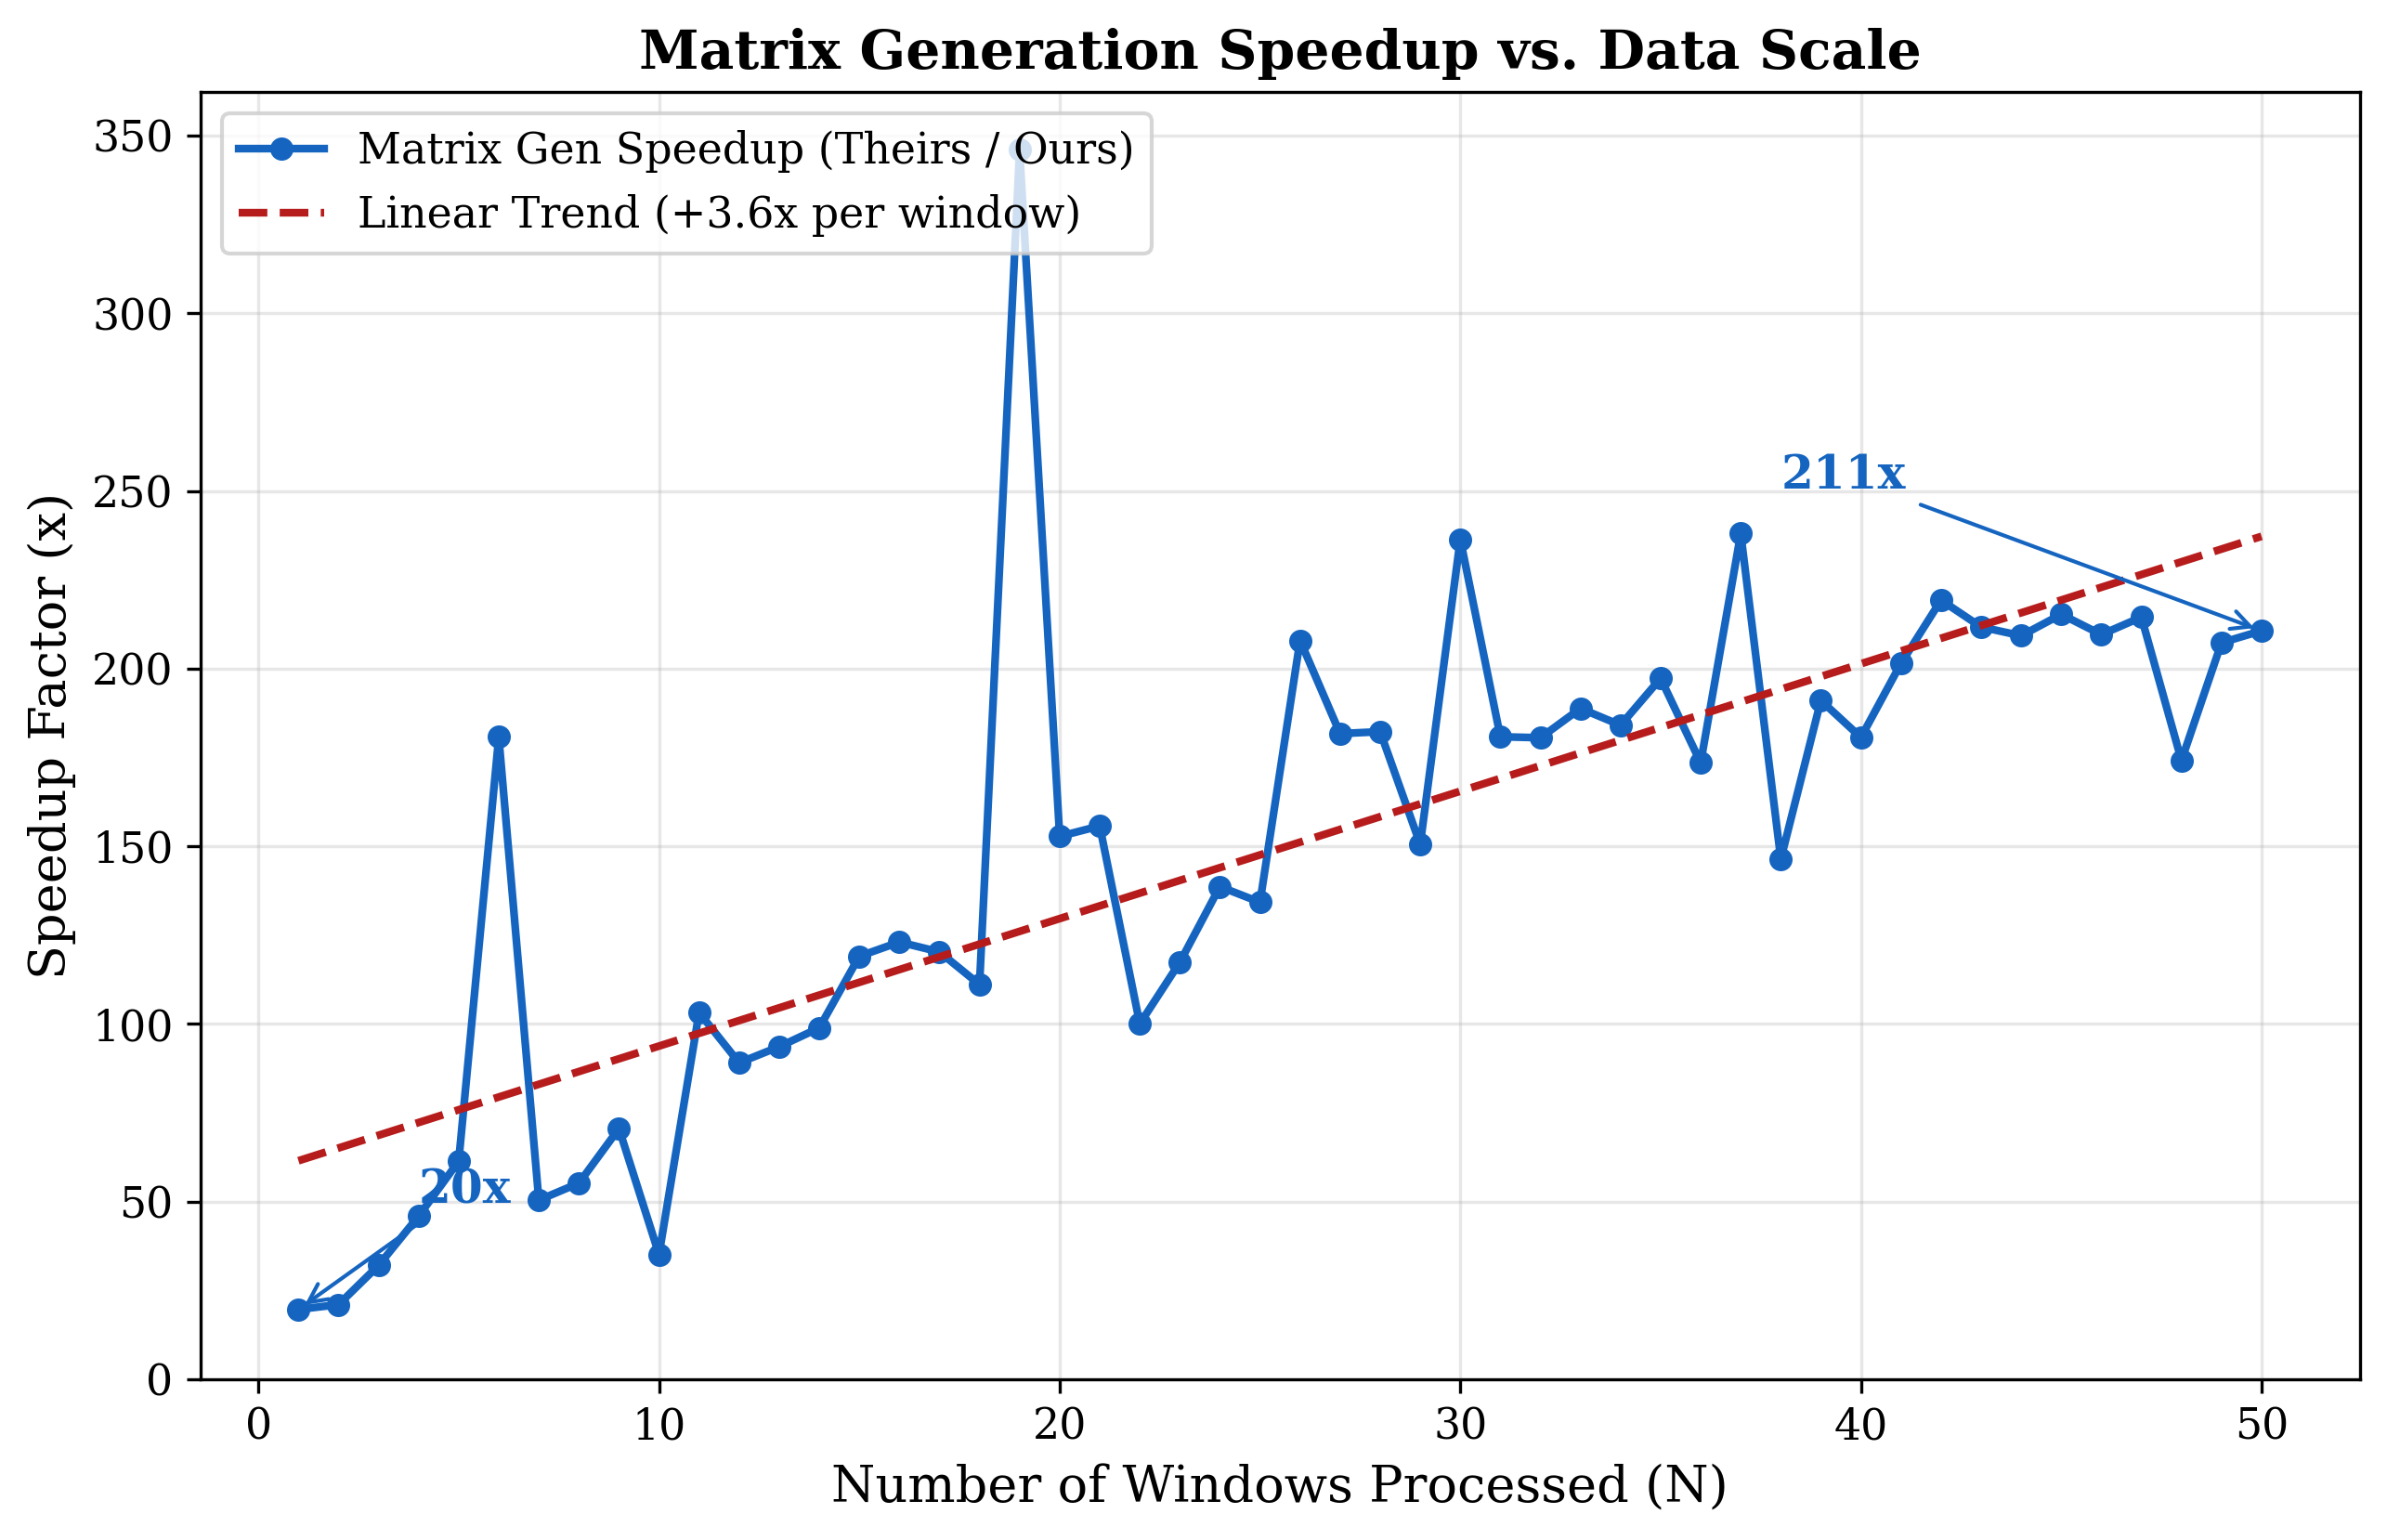
\includegraphics[width=0.8\linewidth]{Evidence/chart_speedup_factor.png}
    \caption{Speedup factor of the relational streaming architecture relative to the batch baseline. The performance gain increases significantly with tracklet density, demonstrating the scalability of the stream-oriented approach.}
    \label{fig:speedup_factor}
\end{figure}

Figure~\ref{fig:speedup_factor} visualizes this divergence. As the number of processed windows increases and the tracklet density grows toward its peak of 556, the performance advantage of the streaming architecture grows from roughly 20$\times$ to over 210$\times$ for the similarity matrix stage alone. This confirms that \textbf{STREAMTRACK} effectively neutralizes the scalability bottleneck that plagues conventional batch-oriented MCPT implementations.

The results confirm that \textbf{STREAMTRACK} achieves a high-performance balance between latency and scalability. The transition to a \textbf{relational streams-and-tables architecture} (\textbf{Ours-Base}) removes the significant bottlenecks associated with similarity matrix generation by leveraging incremental windowing and continuous state management. While batch-oriented pipelines like \textbf{Theirs} are forced to compare all person-hypotheses globally, our system exploits the sparsity of real-world camera networks. 

By defining association as a join over a reconfigurable \texttt{CameraTopologyTable}, we eliminate the "search space explosion" that occurs in conventional MCOT implementations. This makes \textbf{STREAMTRACK} uniquely suited for large-scale urban deployments where the number of cameras can reach the thousands, yet each camera cluster remains small enough for sub-10ms processing. The bottleneck in our system is shifted from algorithmic complexity to local streaming I/O, providing a predictable and stable "Real-Time" guarantee that remains consistent even as the global camera network expands.

The breakthrough in \emph{Similarity Matrix Generation} (156$\times$ average speedup, peaking at 210$\times$ on the NVIDIA SmartSpaces dataset) is specifically attributed to the architectural shift from batch-oriented list processing to \textbf{stream-oriented relational operations} which enable efficient memory locality and incremental updates. At the implementation level, this is further accelerated by the JVM's Just-In-Time (JIT) compilation of compiled primitive floating-point loops, which optimizes loop execution and avoids the boxing/unboxing and interpreter overhead of the dynamically typed reference baseline. Overall, the system achieves a processing time of 516 milliseconds for a 4-camera window in the Woven WTS dataset, demonstrating its robust capability for real-time operation in diverse multi-camera environments.





\section{Discussion}\label{sec:discussion}
\subsection{Benefits of a SQL/Streams-and-Tables Formulation}
Expressing MCOT as continuous queries provides significant operational benefits. \textbf{Inspectability}: Developers can query the \texttt{GlobalIDTable} at runtime using standard SQL to audit association decisions and trace identity assignments. \textbf{Modularity}: New vision operators (e.g., pose estimation) can be integrated by adding new join predicates without modifying the core system architecture. \textbf{Reconfigurability}: Camera neighborhoods can be updated via streams without restarting the pipeline.

\subsection{Limitations and Failure Modes}
Despite the high performance, certain challenges remain. Extremely crowded scenes may still lead to similarity ambiguities that even topological gating cannot resolve. Furthermore, rapid lighting changes or occlusions can cause embedding drift, requiring more sophisticated online re-training of the appearance models—a direction for future work.

\subsection{Deployment Considerations}
The streaming architecture naturally supports edge-to-cloud partitioning. Since the single-camera tracking stage (SCPT) operates independently per camera and emits compact \texttt{SingleCameraResult} events, it can be deployed at the edge, while the topology-aware joins and global clustering are centralized in a CEP engine. Our benchmarks show that the MCPT clustering stage processes a 4-camera window in 516ms (Woven WTS) and a topology-aware group averaging $10.10 \pm 11.11$ ms per call ($9.15 \pm 8.27$ ms excluding JIT warm-up; see Table~\ref{tab:9camera_performance}), confirming that even edge devices with modest compute can handle the centralized association workload. This partitioning reduces backhaul bandwidth from raw video streams to lightweight feature events while maintaining a global view of person identities.

\section{Related Work}\label{sec:related}

\paragraph{Multi-Camera People Tracking: AI City Challenge Baselines.}
The NVIDIA AI City Challenge~\cite{wang2024aicity} has catalyzed high-performing multi-camera people tracking (MCPT) systems. In the 2024 edition (Track~1), the highest-scoring offline entry by Yoshida et al.~\cite{yoshida2024overlap} (RIIPS/Yachiyo, achieving the highest raw HOTA of 71.94\%) proposed an \emph{offline} framework built on a custom \emph{Overlap Suppression Clustering} (OSC) algorithm. OSC leverages future-frame context to retrospectively resolve overlap anomalies---cases where a single tracklet erroneously contains detections from multiple identities occupying the same frame---using weighted degree centrality for bipartite re-assignment. For cross-camera Re-ID, they categorize detections into three confidence levels (Lv.3/2/1) based on HRNet pose estimation keypoints, select representative images from the highest available level, and cluster them via average-linkage hierarchical clustering on a similarity matrix refined by world-coordinate Euclidean distances. Low-identifiability tracklets are assigned to existing clusters as a final post-processing step. Our system takes this exact pipeline as the functional baseline and re-architects it as a streaming program, achieving 100\% Global ID parity and $<10^{-6}$ MAD in similarity matrices \emph{online}, without requiring offline post-processing.

Among online challenge entrants, Kim et al.~\cite{kim2024cluster} (Nota, 3rd place, with a raw HOTA score of 60.93\%) proposed \emph{Cluster Self-Refinement} (CSR), which periodically executes agglomerative clustering to split tracklets contaminated with mixed-identity features, and merges duplicate global IDs by comparing spatial-visual distances. They further leverage RTMPose for angle-aware ground-plane projection (updating camera-specific interpolation ratios via exponential moving average) and filter occluded bounding boxes via Procrustes shape analysis to ensure diverse, high-quality appearance features in each tracklet. Xie et al.~\cite{xie2024robust} (SJTU-Lenovo, 2nd place in raw HOTA score of 67.22\% but the overall Track~1 winner after the 10\% online tracking bonus) combined geometric consistency constraints with state-aware Re-ID correction to handle camera handoffs. Specker~\cite{specker2024ocmctrack} (OCMCTrack, 4th place, with a raw HOTA score of 60.88\%) introduced a corrective matching cascade consisting of track splitting (to prune false-positive associations based on visual similarity thresholds), position-based hierarchical clustering, adapted projection-line matching (to handle bounding boxes truncated at frame borders), and Re-ID-based rematching for lost tracks. Yang et al.~\cite{yang2024online} (UW-ETRI, 5th place, raw HOTA score of 57.14\%) decoupled spatial association (clustering multi-camera foot-point projections) from temporal tracking (world-coordinate Kalman filtering), but relied heavily on offline post-processing---tracklet splitting via inner cosine feature distance and hierarchical merging---to correct cumulative online errors.

Unlike these approaches, \textbf{STREAMTRACK} does not employ global per-frame bipartite matching cascades or separate offline correction passes. Instead, we express the association logic as continuous SQL/EPL queries over relational state tables (\texttt{GlobalIDTable}, \texttt{CameraTopologyTable}). Identity switches and stale tracks are resolved incrementally via priority-ordered EPL timer queries, and the search space is pruned from global $O(N^2)$ comparisons to $O(N)$ locally via topology-aware stream joins---preserving absolute functional accuracy while delivering a 34$\times$ overall speedup.

\paragraph{Online vs.\ Offline Tracking and Scalability.}
Multi-camera tracking systems are broadly classified as \emph{offline} (batch) or \emph{online} (incremental). Offline methods~\cite{yoshida2024overlap} leverage global optimization over entire video sequences, exploiting future frames for higher accuracy but at latencies that preclude real-time deployment. Online methods~\cite{kim2024cluster,xie2024robust,specker2024ocmctrack} process observations causally, yet even these ``online'' solutions typically rely on internal batch windows for cross-camera association, accumulating detections over fixed intervals before performing global clustering. Critically, \emph{scalability} in the MCPT literature is almost exclusively treated as a computer-vision concern (handling denser crowds, more detections) rather than a \emph{systems} concern (adding cameras, reconfiguring topology, maintaining state under growth). Our work is orthogonal to these accuracy-centric advances: we take an existing offline pipeline and re-architect it as a streaming program, preserving its functional output while gaining systems-level properties---scalability via topology-aware partitioning ($4.16\times$ latency reduction at 9 cameras, or $4.27\times$ in steady state), inspectability via queryable state tables, and reconfigurability via live topology updates (464\,ms reconfiguration with zero downtime).

\paragraph{Industrial Video Analytics Frameworks.}
NVIDIA DeepStream~\cite{nvidia2024deepstream} is the dominant industrial SDK for GPU-accelerated video analytics. Built on GStreamer, it provides a modular pipeline of hardware-accelerated plugins for decoding, inference, and single-camera tracking (NvDCF, DeepSORT, IOU). However, its native trackers operate within a single camera stream; cross-camera identity association requires an external microservice layer. NVIDIA Metropolis~\cite{nvidia2025metropolis} addresses this gap with a Kubernetes-based reference architecture that decomposes multi-camera tracking into containerized microservices communicating via message brokers. While Metropolis provides a scalable deployment model, it remains a heavyweight, opaque infrastructure: association logic is embedded in compiled services rather than expressed as declarative queries, intermediate tracking state is not directly queryable for debugging, and reconfiguring the camera network typically requires container re-deployment or manual API calls rather than a single streaming event. In contrast, \textbf{STREAMTRACK} expresses association as parameterized SQL/EPL joins over a relational topology table, enabling zero-downtime reconfiguration, SQL-based state inspection, and a lightweight single-process deployment.

\paragraph{Stream Processing Foundations and CEP Engine Selection.}
Our architectural approach draws from the streams-and-tables duality formalized by Sax et al.~\cite{sax2018streams}. Apache Kafka~\cite{kreps2011kafka} and its Kafka Streams library operationalized this duality via KTables and changelog topics, enabling stateful stream processing at scale, though without native support for the windowed join semantics and complex event sequence patterns required by vision workloads. Apache Flink~\cite{carbone2015flink} provides a more expressive model with native CEP pattern detection, event-time watermarks, and exactly-once guarantees, but introduces significant infrastructure complexity (cluster deployment, checkpoint management) and network serialization overhead when transferring high-dimensional visual feature tensors across distributed worker nodes. Furthermore, Flink's static operator graph makes zero-downtime query redeployment---required when the camera topology changes---extremely costly, as it necessitates stopping the job, modifying the DAG, and restarting from a savepoint.

Our implementation uses Esper~\cite{espertech2024}, a mature CEP engine that combines SQL-like continuous queries (EPL) with full relational table semantics in an embeddable, single-process JVM runtime. By running within the application process, Esper enables zero-overhead sharing of heavy appearance feature tensors between tracking operators and state tables, avoiding the serialization/deserialization costs inherent in distributed engines. Esper's API further supports compiling, deploying, and undeploying EPL statements at runtime, which directly enables our reactive topology reconfiguration loop.

The closest prior work applying CEP to video analytics is VidCEP~\cite{yadav2019vidcep}, which introduced a graph-based Video Event Knowledge Graph (VEKG) and a Video Event Query Language (VEQL) for detecting spatiotemporal patterns (e.g., ``Red Car Left of Person'', loitering, traffic flow) in video streams. As analyzed in VidCEP, existing Event Query Languages (such as Snoop~\cite{chakravarthy1994snoop}, SASE~\cite{wu2006sase}, TESLA~\cite{cugola2010tesla}, and Cayuga~\cite{demers2007cayuga}) are designed for temporal sequence matching on alphanumeric event streams and lack the ability to process high-dimensional video streams or reason about spatial relationships. On the other hand, database-oriented video query languages (such as VSQL~\cite{10.1145/951676.951682}, MOQL~\cite{li1997moql}, BilVideo~\cite{donderler2005bilvideo}, SVQL~\cite{lu2015svql}, and CVQL~\cite{le2008query}) support object, attribute, and spatial relationship queries, but are strictly built for batch querying of offline, pre-annotated databases, failing to handle continuous, real-time streaming joins. VidCEP addresses this by extending Esper with external deep learning frameworks to populate a graph-based event model. However, VidCEP targets \emph{post-tracking event and anomaly detection}---recognizing high-level behavior patterns from already-segmented and tracked object trajectories---rather than the structurally distinct problem of \emph{multi-camera identity tracking (MCOT)}. MCOT requires continuously maintaining a mutable table of active identity mappings (\texttt{GlobalIDTable}), resolving coordinate projections, and executing topology-aware joins in real time. We choose Esper because it serves as a high-performance relational coordinator: we do not attempt to represent raw pixels or neural network inference inside the declarative query language itself; rather, we offload vision kernels (Re-ID, projection) to modular operators and use Esper to orchestrate stream windowing, relational state maintenance, and topological gating. To our knowledge, no prior work has applied the streams-and-tables paradigm to the core MCOT pipeline itself.

\paragraph{Summary and Gap.}
The literature reveals a clear gap at the intersection of multi-camera tracking and stream processing systems. CV-oriented works~\cite{yoshida2024overlap,kim2024cluster,xie2024robust,specker2024ocmctrack,yang2024online} focus on improving tracking heuristics but treat the processing architecture as a fixed implementation detail. Industrial frameworks~\cite{nvidia2024deepstream,nvidia2025metropolis} provide scalable deployment but lack declarative association logic, queryable state, and zero-downtime reconfigurability. Stream processing systems~\cite{sax2018streams,carbone2015flink,kreps2011kafka} and video CEP frameworks~\cite{yadav2019vidcep} provide theoretical and practical foundations for continuous data processing but have not been applied to the core MCOT pipeline. \textbf{STREAMTRACK} bridges this gap by formulating multi-camera tracking as a relational streaming program in which identity is a continuously maintained table, association is a parameterized stream join, and the camera topology is a reconfigurable state relation.

\section{Conclusion and Future Work}\label{sec:conclusion}
We presented \textbf{STREAMTRACK}, a relational streams-and-tables architecture for multi-camera object tracking. By recasting MCOT as a continuous query problem and utilizing topology-aware stream joins, we achieved a \textbf{156$\times$ average speedup} in similarity generation and a \textbf{34$\times$ overall speedup} over batch-oriented baselines on the NVIDIA SmartSpaces dataset. Scaling the NVIDIA SmartSpaces network with topology-aware partitioning yields a further \textbf{4.16$\times$} (up to \textbf{4.27$\times$} in steady state excluding JVM warm-up) latency reduction per association call. Our system ensures real-time performance even as the camera network grows, while providing an architecture that supports unique operational benefits like runtime reconfigurability and SQL-based inspectability.

\paragraph{Future work.}
Future directions include: (i) multi-hop topology reasoning, where cameras beyond immediate neighbors contribute to association via transitive similarity; and (ii) learning topology weights from historical data to dynamically adjust join selectivity.

\bibliographystyle{plain}
\bibliography{references}

\end{document}
